\documentclass[11pt,spanish]{article} % Tipo y tamaño de letra del documento.


\usepackage[utf8]{inputenc}
\usepackage{subfiles}
\usepackage{biblatex}
\addbibresource{references.bib}
\usepackage{multicol}
\usepackage{amsfonts}
\usepackage{blindtext}
\usepackage{mathrsfs}
\usepackage{amsmath}
\usepackage{siunitx}
\usepackage{centernot}
\usepackage[shortlabels]{enumitem}
\usepackage{subfig}
\usepackage{datetime}
\usepackage{listingsutf8}
\usepackage[spanish]{babel}
\usepackage{tikz}
\usepackage{hyperref}
\usepackage[vlined,ruled,linesnumbered]{algorithm2e}
\usepackage{listings}
\usepackage{float}
\usepackage{url}
\usepackage{csquotes}
\usepackage{fourier} %font
\usepackage[top=2cm, bottom=2cm, left=2.5cm, right=2.5cm]{geometry}
\usepackage{pgfplots}
\usepackage{fancyhdr}
\usepackage{mdframed}
\usepackage{tikzducks}
\usepackage[nameinlink]{cleveref}
\usepackage{epigraph} 

\pgfplotsset{compat=1.18}

\usetikzlibrary{shapes.arrows, shapes.geometric, arrows.meta,angles,quotes,positioning,arrows,fit,quotes,calc}
\tikzset{>=latex} 

\setlength\algomargin{1em} 
\SetFuncSty{sc} 
\SetCommentSty{em} 


\Crefname{figure}{Fig.}{Figs.}
\newcommand\crefrangeconjunction{--}
\Crefname{table}{Tabla}{Tablas}
\Crefname{subsubsection}{Subsubsec.}{Subsubsections}
\Crefname{subsection}{Subsec.}{Subsections}
\Crefname{section}{Sec.}{Sections}
\Crefname{equation}{eq.}{eqs.}
\crefname{thm}{Theorem}{theorems}
\Crefname{thm}{Theorem}{Theorems} 

\definecolor{algoco}{rgb}{0,0.4,1}

\hypersetup{
  colorlinks=true,
  linkcolor=algoco,
  citecolor=blue,
  urlcolor=blue,
}

\lstset{
extendedchars=true
inputencoding=utf8/latin1,
basicstyle=\footnotesize\sffamily\color{black},
commentstyle=\slshape \color{gray},
numbers=left,
numbersep=10pt,
numberstyle=\tiny\color{red!80!black},
keywordstyle=\color{red!80!magenta},
showspaces=false,
showstringspaces=false,
stringstyle=\color{cyan!80!black},
tabsize=2,
literate={á}{{\'a}}1 {é}{{\'e}}1 {í}{{\'i}}1 {ó}{{\'o}}1 {ú}{{\'u}}1,
frame = single, 
numbers = none,
float, floatplacement = ht, captionpos = b,
xleftmargin = 2em, xrightmargin = 2em, 
}

\newcommand{\ub}[1]{\underbrace{#1}}
\newcommand\tcm{\textcolor{magenta}}
\newcommand\tca{\textcolor{algoco}}

\setlength\epigraphwidth{.7\textwidth} 

\newcommand{\tnum}{2 y 3} % reemplace 2 por el número de la tarea
\newcommand{\sem}{2024-2} % reemplace 2024-2 por el semestre correspondiente
\newcommand{\campus}{San Joaquin \\ Santiago} % reemplace Casa Central por el campus correspondiente
\newcommand{\rolusm}{202273615-1} % reemplace 2025073100-1 por su rol
\newcommand{\namestudent}{Andrés Águila Montenegro} % reemplace Al Goritmo Pérez por su nombre

\headheight=14pt
\linespread{1.3}
\author{\namestudent}
\pagestyle{fancy}
\fancyhf{}%
\fancyfoot[R]{ \namestudent \\ \rolusm}
\fancyfoot[L]{Campus \campus} 
\fancyfoot[C]{\thepage}
\rhead{2024-2}
\lhead{INF-221}
\renewcommand{\headrulewidth}{0.4pt}
\renewcommand{\footrulewidth}{0.4pt}
\newbool{programs}
\boolfalse{programs}
\chead{REPORTE TAREA \tnum~}



\title{
  \huge
  \textbf{REPORTE TAREA \tnum~ \\ ALGORITMOS Y COMPLEJIDAD} \\[1ex]
  \emph{\textquote{Explorando la Distancia entre Cadenas, una Operación a la Vez}}
  }

  
\date{
  \small
  \today\\
  \currenttime
}




\begin{document}
\maketitle
\thispagestyle{fancy} 
\vspace{-1.0\baselineskip}




\begin{abstract}
  \textit{ 
    Un resumen es un breve compendio que sintetiza todas las secciones clave de un trabajo de investigación: la introducción, los objetivos, la infraestructura y métodos, los resultados y la conclusión. Su objetivo es ofrecer una visión general del estudio, destacando la novedad o relevancia del mismo, y en algunos casos, plantear preguntas para futuras investigaciones. El resumen debe cubrir todos los aspectos importantes del estudio para que el lector pueda decidir rápidamente si el artículo es de su interés.

En términos simples, el resumen es como el menú de un restaurante que ofrece una descripción general de todos los platos disponibles. Al leerlo, el lector puede hacerse una idea de lo que el trabajo de investigación tiene para ofrecer \cite{elsevier_abstract_2024}.

\textbf{La extensión del resumen, para esta entrega, debe ser tal que la totalidad del índice siga apareciendo en la primera página. Recuerde que NO puede modificar el tamaño de letra, interlineado, márgenes, etc.}

  }
     
\end{abstract}

\setcounter{tocdepth}{1}
\tableofcontents


\newpage
\section{Introducción}
\begin{mdframed}
    \textbf{La extensión máxima para esta sección es de 2 páginas.}
\end{mdframed}

La introducción de este tipo de informes o reportes, tiene como objetivo principal \textbf{contextualizar el problema que se va a analizar}, proporcionando al lector la información necesaria para entender la relevancia del mismo. 

Es fundamental que en esta sección se presenten los antecedentes del problema, destacando investigaciones previas o principios teóricos que sirvan como base para los análisis posteriores. Además, deben explicarse los objetivos del informe, que pueden incluir la evaluación de un algoritmo, la comparación de métodos o la validación de resultados experimentales.

Aunque la estructura y el enfoque siguen principios de trabajos académicos, se debe recordar que estos informes no son publicaciones científicas formales, sino trabajos de pregrado. Por lo tanto, se busca un enfoque claro y directo, que permita al lector comprender la naturaleza del problema y los objetivos del análisis, sin entrar en detalles excesivos. 


Introduction Checklist de \citetitle{GoodScientificPaper} \cite{GoodScientificPaper}, adaptada a nuestro contexto:

\begin{itemize}
\item Indique el \textbf{campo del trabajo} (Análisis y Diseño de algoritmos en Ciencias de la Computación), por qué este campo es importante y qué se ha hecho ya en este área, con las \textbf{citas} adecuadas de la literatura académica o fuentes relevantes.
\item Identifique una \textbf{brecha} en el conocimiento, un desafío práctico, o plantee una \textbf{pregunta} relacionada con la eficiencia, complejidad o aplicabilidad de un algoritmo particular.
\item Resuma el propósito del informe e introduzca el análisis o experimento, dejando claro qué se está investigando o comparando, e indique \textbf{qué es novedoso} o por qué es significativo en el contexto de un curso de pregrado.
\item Evite; repetir el resumen; proporcionar información innecesaria o fuera del alcance de la materia (limítese al análisis de algoritmos o conceptos de complejidad); exagerar la importancia del trabajo (recuerde que se trata de un informe de pregrado); afirmar novedad sin una comparación adecuada con lo enseñado en clase o la bibliografía recomendada.
\end{itemize}



\begin{mdframed}
Recuerde que este es su trabajo, y sólo usted puede expresar con precisión lo que ha aprendido y quiere transmitir. Si lo hace bien, su introducción será más significativa y valiosa que cualquier texto automatizado. ¡Confíe en sus habilidades, y verá que puede hacer un mejor trabajo que cualquier herramienta que automatiza la generación de texto!
\end{mdframed}



\newpage
\section{Diseño y Análisis de Algoritmos} 
\begin{mdframed}
    \textbf{La extensión máxima para esta sección es de 5 páginas.}
\end{mdframed}




\subsection{Fuerza Bruta}

%\epigraph{\textit{``Indeed, brute force is a perfectly good technique in many cases; the real question is, can we use brute force in such a way that we avoid the worst-case behavior?''}}{--- \citeauthor{taocv3}, \citeyear{taocv3} \cite{taocv3}}

\subsubsection{Descripción de la solución}
Resolver el problema de distancia de edición utilizando el enfoque de fuerza bruta no tiene gran complejidad en su diseño.
Buscamos igualar s1 a s2 probando todas las combinaciones posibles que surgen a partir de las 4 operaciones que dicta el problema.
Para este ejemplo se compara recursivamente y de manera ascendente los elementos de s1 y s2 con ayuda de índices ($i$ y $j$).
Por cada par de caracteres ubicados en s1[i] y s2[j], se evaluan en casos separados las cuatro acciones posibles a realizar
con ambos elementos, agregando el costo relacionado con la operación. Cada caso representaría una \textit{``ruta''} por la cual se buscaría llegar a la solución.
Luego de calcular cada uno de los casos, se escoje el de menor costo, retornando el costo óptimo de cada subtarea y, finalmente, el costo óptimo del problema original.
\subsubsection{Algoritmo utilizando fuerza bruta}
\begin{algorithm}[H]
    \SetKwProg{myproc}{Procedure}{}{}
    \SetKwFunction{BruteForce}{bruteForce}
    \SetKwFunction{CostInsert}{costInsert}
    \SetKwFunction{CostDelete}{costDelete}
    \SetKwFunction{CostSubstitute}{costSubstitute}
    \SetKwFunction{CostTranspose}{costTranspose}
    
    \DontPrintSemicolon
    \footnotesize

    \myproc{\BruteForce{s1, s2, i, j}}{
        \uIf{i = longitud(s1) \textbf{ and } j = longitud(s2)}{
            \Return 0  \tcp*[r]{Ambas cadenas están completas}
        }
        \uElseIf{i = longitud(s1)}{
            \Return (\CostInsert{s2[j]} + \BruteForce{s1, s2, i, j + 1})  \tcp*[r]{Insertar restante de s2}
        }
        \uElseIf{j = longitud(s2)}{
            \Return (\CostDelete{s1[i]} + \BruteForce{s1, s2, i + 1, j})  \tcp*[r]{Eliminar restante de s1}
        }
        
        \tcp{Calcula el costo mínimo entre las operaciones posibles}
        $costo_{del} \leftarrow \CostDelete{s1[i]} + \BruteForce{s1, s2, i + 1, j}$\;
        $costo_{ins} \leftarrow \CostInsert{s2[j]} + \BruteForce{s1, s2, i, j + 1}$\;
        $costo_{sub} \leftarrow \CostSubstitute{s1[i], s2[j]} + \BruteForce{s1, s2, i + 1, j + 1}$\;
        
        $costo_{trans} \leftarrow \infty$\;
        \uIf{i + 1 $<$ largo s1 \textbf{ and } j + 1 $<$ largo s2 \textbf{ and } s1[i] = s2[j+1] \textbf{ and } s1[i+1] = s2[j]}{
            $costo_{trans} \leftarrow \CostTranspose{s1[i], s1[i+1]} + \BruteForce{s1, s2, i + 2, j + 2}$\;
            }
            
        \Return $\min(costo_{del}, costo_{ins}, costo_{sub}, costo_{trans})$\;
    }

    \myproc{\CostInsert{b}}{
        \Return costo de inserción para `$b$` \tcp*[r]{Función de costo de inserción}
    }
    \myproc{\CostDelete{a}}{
        \Return costo de eliminación para `$a$` \tcp*[r]{Función de costo de eliminación}
    }
    \myproc{\CostSubstitute{a, b}}{
        \Return costo de sustitución entre `$a$` y `$b$` \tcp*[r]{Función de costo de sustitución}
    }
    \myproc{\CostTranspose{a, b}}{
        \Return costo de transposición entre `$a$` y `$b$` \tcp*[r]{Función de costo de transposición}
    }
    \caption{Algoritmo de Fuerza Bruta para calcular la distancia mínima de edición}
    \label{alg:bruteforce_edit_distance}
\end{algorithm}


\subsubsection{Ejemplo de ejecución}
Vamos a simular la ejecución del algoritmo diseñado con los datos de entrada s1: ``dog'' y s2: ``bag''.

\textbf{Paso 1:}:

// Se checkea si es un caso base

\begin{tabbing}
    $costo_{del} \leftarrow \CostDelete{s1[i]} + \BruteForce{s1, s2, i + 1, j}$\;


    \textbf{Vuelve al paso 1 con otros parámetros}:
\end{tabbing}

\begin{tabbing}
    $costo_{ins} \leftarrow \CostInsert{s2[j]} + \BruteForce{s1, s2, i, j + 1}$\;


    \textbf{Vuelve al paso 1 con otros parámetros}:
\end{tabbing}

\begin{tabbing}
    $costo_{sub} \leftarrow \CostSubstitute{s1[i], s2[j]} + \BruteForce{s1, s2, i + 1, j + 1}$\;


    \textbf{Vuelve al paso 1 con otros parámetros}:
\end{tabbing}

// Solo si es que se cumple la condición
\begin{tabbing}
    $costo_{trans} \leftarrow \CostTranspose{s1[i], s1[i+1]} + \BruteForce{s1, s2, i + 2, j + 2}$\;


    \textbf{Vuelve al paso 1 con otros parámetros}:
\end{tabbing}

\textbf{Paso 2:}

Al finalizar todas las llamadas recursivas se evaluan los resultados con:

\begin{tabbing}
    $\min(costo_{del}, costo_{ins}, costo_{sub}, costo_{trans})$
\end{tabbing}

y se retorna a la llamada anterior, para que esta \textbf{repita el paso 2} o en su defecto, retorne el valor a la llamada original, resolviendo el problema.


\subsubsection{Complejidad temporal y espacial}
En cada instancia de este algoritmo, este realiza al menos 3 llamadas recursivas a si mismo. La cuarta llamada ocurre en casos donde sea posible llevar a cabo esta operación, 
por ende, tomando en cuenta esta situación como el peor caso, el algoritmo tendría 4 llamadas recursivas. 

En caso de que un string sea mas largo que el otro, se llega a un caso base que, si bien tambien ejecuta una llamada
recursiva, esta solo realizaría acciones de complejidad lineal, por lo que las llamadas recursivas masivas del algoritmo 
\textbf{se detienen al alcanzar el tamaño del string más corto.} 

Si tuvieramos que combinar $n$ elementos de 4 maneras distinas, tendríamos $4^n$ combinaciones, siguiendo
este ejemplo y ya que este algoritmo evalúa todas las posibles combinaciones hasta el tamaño del string más pequeño, el enfoque fuerza bruta tiene 
una complejidad temporal de $O(4^{\min(n,m)})$, con $n$ y $m$ los largos de s1 y s2, respectivamente. 

En cuanto a la complejidad espacial, este algoritmo no ocupa ningún tipo de memoria adicional. Al ser in-place este tiene una complejidad espacial
de $O(1)$.


\subsubsection{Inclusión de Transposición y costos variables}
La inclusión de la acción de transposición al problema original añade un grado mayor de complejidad al problema. Esto aumenta la cantidad de llamadas
recursivas, empeorando considerablemente el rendimiento con respecto al problema sin esta opción. Los casos que presenten un mayor impacto debido a esta 
complejidad extra son aquellos donde la acción de ``transponer'' sea posible para todo el string, forzando que en cada llamada al algoritmo se ejecuten 
los 4 casos recursivos.

Con respecto a los costos variables, estos no afectan directamente la complejidad, ya que cada valor se recuperaría en tiempo constante a través de las funciones 
auxiliares.
\subsection{Programación Dinámica}

%\epigraph{\textit{Dynamic programming is not about filling in tables. It's about smart recursion!}}{\citeauthor{algorithms_erickson}, \citeyear{algorithms_erickson} \cite{algorithms_erickson}}

%\begin{enumerate}[1)]
%    \item Describa la solución recursiva.
%    \item Escriba la relación de recurrencia, incluyendo condiciones y casos base.
%    \item Identifique subproblemas.
%    \item Defina estructura de datos a utilizar y especifique el orden de calculo que realiza su programa que utiliza programación dinámica. 
%\end{enumerate}

\subsubsection{Descripción de la solución recursiva}
Este enfoque se centra en hallar la solución óptima sin realizar recusión innecesaria. Para lograrlo, utlizaremos programación dinámica con el método bottom-up:
precalcularemos las soluciones óptimas de los subproblemas de manera iterativa y lo almancenaremos en una matriz caché ($dp$). Como veremos en los siguientes puntos,
el llenado de la tabla se hará según la relación de recurrencia para al finalizar poder encontrar el óptimo del problema original en la casilla con las mayores coordenadas.

\subsubsection{Relación de recurrencia}

\begin{equation}
    dp_{s1,s2}(i,j)=\min\begin{cases}
      0, & \text{if i = j = 0},\\
      dp_{s1,s2}(i-1,j) + costDel(s1_{i}) & \text{if $i > 1$},\\
      dp_{s1,s2}(i,j-1) + costIns(s2_{j}) & \text{if $j > 1$},\\
      dp_{s1,s2}(i-1,j-1) + costSust(s1_{i},s2{j}) & \text{if $i,j > 1$},\\
      dp_{s1,s2}(i-2,j-2) + costTrsp(s1_{i},s1_{i-1}) & \text{if $i,j > 1 $ and $ s1_{i} = s2_{j-1}$ and $s1_{i-1} = s2_{j}.$}
    \end{cases}
\end{equation}
\subsubsection{Identificación de subproblemas}
Cada subproblema se identifica por dos elementos, el último elemento de s1 y el último elemento de s2. Este enfoque busca resolver todos los posibles subproblemas 
de manera creciente, es decir, empezando desde s1 y s2 sin elementos, pasando por s1 con i elementos y s2 con j elementos, hasta llegar al problema de s1 y s2 completos, 
siendo esta la pregunta original.
\subsubsection{Estructura de datos y orden de cálculo}
La creación de la tabla $dp$ implica utilizar un arreglo bidimensional, es decir, un arreglo de arreglos y para la visualización de la tabla, vamos a considerar la esquina (0,0) como superior-izquierda. 

Como pudimos ver en la relacion de recurrencia, la respuesta de cada problema es el óptimo entre 4 subproblemas menores. 
Cada una de estas respuestas se encuentra arriba, a la izquierda o en diagonal superior-izquierda respecto a el problema actual, por lo que cada cálculo tiene como requisito que las casillas en esas direcciones ya tengan un valor asignado. Esto hace que, luego de rellenar los casos 
base \textit{(fila 0 para s2 vacío y columna 0 para s1 vacío)}, podamos calcular cada casilla de izquierda a derecha y de arriba hacia abajo.
\subsubsection{Algoritmo utilizando programación dinámica}



\begin{algorithm}[H]
    \SetKwProg{myproc}{Procedure}{}{}
    \SetKwFunction{Dynamic}{dynamic}
    \SetKwFunction{CostInsert}{costInsert}
    \SetKwFunction{CostDelete}{costDelete}
    \SetKwFunction{CostSubstitute}{costSubstitute}
    \SetKwFunction{CostTranspose}{costTranspose}
    
    \DontPrintSemicolon
    \footnotesize

    \myproc{\Dynamic{s1, s2}}{
        \tcp{Inicializa matriz de costos}
        Crear matriz $dp$ de dimensiones (longitud(s1)+1) x (longitud(s2)+1)\;
        \tcp{Rellenado de casos base}
        $dp[0][0] \leftarrow 0$\;
        \For{$i \leftarrow 1$ \KwTo longitud(s1)}{
            $dp[i][0] \leftarrow i \times \CostDelete{s1[i-1]}$ \tcp*[r]{Costo de borrar lo que sobra de s1}
        }
        \For{$j \leftarrow 1$ \KwTo longitud(s2)}{
            $dp[0][j] \leftarrow j \times \CostInsert{s2[j-1]}$ \tcp*[r]{Costo de insertar lo que falta de s2}
        }

        \For{$i \leftarrow 1$ \KwTo longitud(s1)}{
            \For{$j \leftarrow 1$ \KwTo longitud(s2)}{
                $costo_{del} \leftarrow dp[i-1][j] + \CostDelete{s1[i-1]}$\;
                $costo_{ins} \leftarrow dp[i][j-1] + \CostInsert{s2[j-1]}$\;
                $costo_{sub} \leftarrow dp[i-1][j-1] + \CostSubstitute{s1[i-1], s2[j-1]}$\;

                $costo_{trans} \leftarrow \infty$\;
                \uIf{i > 1 \textbf{ and } j > 1 \textbf{ and } s1[i-1] = s2[j-2] \textbf{ and } s1[i-2] = s2[j-1]}{
                    $costo_{trans} \leftarrow dp[i-2][j-2] + \CostTranspose{s1[i-2], s1[i-1]}$\;
                }
                $dp[i][j] \leftarrow \min(costo_{del}, costo_{ins}, costo_{sub}, costo_{trans})$\;
            }
        }
        
        \Return $dp[\text{longitud(s1)}][\text{longitud(s2)}]$\;
    }

    \myproc{\CostInsert{b}}{
        \Return costo de inserción para `$b$` \tcp*[r]{Función de costo de inserción}
    }
    \myproc{\CostDelete{a}}{
        \Return costo de eliminación para `$a$` \tcp*[r]{Función de costo de eliminación}
    }
    \myproc{\CostSubstitute{a, b}}{
        \Return costo de sustitución entre `$a$` y `$b$` \tcp*[r]{Función de costo de sustitución}
    }
    \myproc{\CostTranspose{a, b}}{
        \Return costo de transposición entre `$a$` y `$b$` \tcp*[r]{Función de costo de transposición}
    }
    \caption{Algoritmo de Programación Dinámica para calcular la distancia mínima de edición}
    \label{alg:dynamic_edit_distance}
\end{algorithm}

\subsubsection{Ejemplo de ejecución}
Vamos a simular la ejecución del algoritmo diseñado con los datos de entrada s1: ``dog'' y s2: ``bag''.

\textbf{1. Rellenamos los casos base}: Asumiendo que todos los costos de inserción = 1 y borrado = 2.

\begin{table}[h]
    \centering
    \begin{tabular}{|c|c|c|c|}
    \hline
    0 & 2 & 4 & 6 \\ \hline
    1 &   &   &   \\ \hline
    2 &   &   &   \\ \hline
    3 &   &   &   \\ \hline
    \end{tabular}
\end{table}

\textbf{2. Rellenaremos una casilla no-base}: Seguiremos los pasos para rellenar (1,1)

$i = 1, j = 1$



\begin{tabbing}
    $costo_{del} \leftarrow dp[i-1][j] + \CostDelete{s1[i-1]}$ = $costo_{del} \leftarrow 2 + 2$\;
\end{tabbing}


\begin{tabbing}
    $costo_{ins} \leftarrow dp[i][j-1] + \CostInsert{s2[j-1]} $ = $ costo_{ins} \leftarrow 1 + 1$\;
\end{tabbing}


\begin{tabbing}
    $costo_{sub} \leftarrow dp[i-1][j-1] + \CostSubstitute{s1[i-1], s2[j-1]}$ = $costo_{sub} \leftarrow 0 + 2$\;
\end{tabbing}

// Costo trans no lo contamos porque no cumple las condiciones

$dp[1][1] \leftarrow \min(4, 2, 2)$ = $dp[1][1] \leftarrow 2$

\begin{table}[h]
    \centering
    \begin{tabular}{|c|c|c|c|}
    \hline
    0 & 2 & 4 & 6 \\ \hline
    1 & 2 &   &   \\ \hline
    2 &   &   &   \\ \hline
    3 &   &   &   \\ \hline
    \end{tabular}
\end{table}

Y así continuariamos con el rellenado de todas las tablas de izquierda a derecha y desde arriba hacia abajo. 
El valor óptimo se encontrará en (3,3).


\subsubsection{Complejidad temporal y espacial}
La complejidad temporal de este algoritmo recae en el tiempo de rellenado de la tabla caché, lo que se realiza a través de dos ciclos \textit{for} anidados.
Teniendo en cuenta que estos ciclos iteran sobre todos los subproblemas posibles, la complejidad temporal de resolver el problema 
a través del algoritmo propuesto es de $O(n*m)$, con $n,m = \textit{tamaño s1 + 1 y tamaño s2 + 1}$, respectivamente. 
\textit{Nótese que para n = m el algoritmo es $O(n^2)$, por lo que se podría decir que es, coloquialmente, un ``algoritmo cuadrático disfrazado''.}   

En cuanto a la complejidad espacial, la memoria extra que se ocupa para esta solución es del tamaño de la tabla $dp$, por ende la complejidad espacial de este algoritmo
es $O(n*m)$.


\subsubsection{Inclusión de Transposición y costos variables}
A diferencia del método de fuerza bruta, la acción extra de transponer no implica un gran impacto en la complejidad, ya que cada una de las operaciones posibles 
dentro del problema tienen un costo de $O(1)$ utilizando este enfoque. Si bien es una mayor carga a que si tuvieramos solo 3 acciones, el impacto de 
sumar una cuarta no es considerable dentro de esta implementación, por ende, a diferencia del anterior, este algoritmo no deberia tener grandes cambios en el tiempo de ejecución 
con strings que permitan constantemente el uso de transposición.

Los costos variables, al igual que en el enfoque anterior, no afectan directamente la complejidad, ya que cada valor se recuperaría en tiempo constante a través de las funciones 
auxiliares.
\newpage
\section{Implementaciones}
Para llevar a cabo los experimentos y las mediciones se utilizaron programas en c++ para los algoritmos, auxiliados por scripts de python para la generación de las tablas de costo, 
datasets, y gráficos en base a los resultados. Los programas se estructuran de la siguiente manera:

\begin{itemize}
    \item \textbf{main.cpp} : programa principal.
    \item \textbf{Aux.hpp} : conjunto de funciones auxiliares, tanto para calcular los costos como para la lectura y escritura de archivos.
    \item \textbf{utilities.hpp} : funciones para mostrar en la terminal el tiempo trasncurrido en cada prueba.
    \item \textbf{BruteForce.hpp} : contiene el algoritmo de fuerza bruta, implementado en c++.
    \item \textbf{dynamicSolution.hpp} : contiene el algoritmo de programación dinámica, implementado en c++.
    \item \textbf{generateCosts.py} : script de python para generar las tablas de costo, se guardan en la carpeta \textit{costs}
    \item \textbf{generateDatasets.py} : script de python para generar los datasets, se guardan en la carpeta \textit{datasets}
    \item \textbf{generateImages.py} : script de python para generar los gráficos, se guardan en la carpeta \textit{imagenes}
\end{itemize}

Además de las carpetas detalladas previamente, deben existir dos carpetas adicionales: \textit{output} y \textit{results}. Asegúrese de que las rutas a 
estas carpetas, así como a las previas, esten correctamente escritas dentro de \textbf{main.cpp} en la función main(), donde existen variables path para 
este propósito. Las carpetas \textit{output} y \textit{results} almacenan los siguientes archivos:

\begin{itemize}
    \item \textbf{/output/outputDetailDp.txt} : archivo de texto que muestra los resultados de las pruebas del algoritmo de programación dinámica. Tiene un formato que facilita la 
    legibilidad. 
    \item \textbf{/output/outputDetailBf.txt} : archivo de texto que muestra los resultados de las pruebas del algoritmo de fuerza bruta. Tiene un formato que facilita la
    legibilidad.
    \item \textbf{/output/outputDp.txt} : archivo de texto que contiene los resultados de las mediciones del algoritmo de programación dinámica de manera comprimida.
    \item \textbf{/output/outputBf.txt} : archivo de texto que contiene los resultados de las mediciones del algoritmo de fuerza bruta de manera comprimida. 
    Estos dos últimos archivos son utilizados para hacer los gráficos mediante \textbf{generateImages.py}.
    \item \textbf{/results/resultsBf.txt}
    \item \textbf{/results/resultsDp.txt}
\end{itemize}
Los dos últimos archivos contienen, junto con sus inputs, los resultados de cada ejecución de los algoritmos correspondientes. Con estos dos archivos es posible comprobar
que ambos algoritmos llegan a un resultado correcto.
Es fundamental que si se quiere utilizar estos programas para la replicación de los experimentos se respete la estructura descrita, con el fin de evitar 
medidas erróneas o fallos de ejecución.

\newpage
\section{Experimentos}

La realización de los experimentos detallados en esta sección fue llevada a cabo bajo las siguientes condiciones:

\begin{itemize}
    \item Hardware:
    \subitem CPU: Ryzen 5 1600, 3.2GHz
    \subitem RAM: 24GB DDR4 2400MHz
    \subitem Almacenamiento: SSD 512GB
    \item Software:
    \subitem {SO: Nobara Linux 40 (KDE Plasma) x86$\_$64}
    \subitem Compilador: g++ 14.2.1
    \subitem Python: 3.12.6
    \subitem Librerías de Python:
    \subsubitem Pandas, Seaborn, matplotlib, Pathlib, Math, Numpy

\end{itemize}

Previo a la realización de las pruebas se cumplieron todos los requisitos para el correcto funcionamiento de los programas 
explicado en la sección anterior. Para ello se poblaron los archivos de costos de operación mediante \textbf{generateCosts.py}.

El problema que buscamos resolver corresponde a la \textit{Distancia de Damerau-Levenshtein} [cita], la cual es frecuentemente usada 
para resolver problemas como el \textit{funcionamiento del autocorrector de un teclado} [cita]. Por ello, para acercarnos a un escenario 
real las tablas de costo se poblaron sus valores asociados según que tan comunes son en el diccionario inglés y que tan probable es un error de typeo 
en función de la distancia entre caracteres en un teclado QWERTY. Esta forma de ajustar los costos determina la forma en la que se reconstruye la 
solución óptima, más no afecta los tiempos de ejecución ni el uso de memoria, los que solo dependen del algoritmo ejecutado y 
las características de los strings de entrada, las cuales dependen de cada dataset. Estos últimos fueron generados mediante \textbf{generateDatasets.py}. 
Las características de cada uno de los datasets se detallan en la siguiente sección.

Cada prueba se llevó a cabo utilizando el programa principal. Cada uno de los casos de prueba se ejecutó 4 veces, midiendo el tiempo de ejecución, el uso de memoria y guardando el resultado. 
Las últimas 3 fueron tomadas en cuenta a la hora de promediar para calcular los valores finales. La primera usa para realizar cualquier tipo de carga de caché que vaya a realizar el programa.

\pagebreak
\subsection{Dataset (casos de prueba)}

Los conjuntos de datos para probar el rendimiento de los algoritmos fueron diseñados para evaluar el comportamiento de estos bajo circunstancias específicas, casos de recursión poco comunes y tambien sus peores casos. 
Los datasets escojidos fueron 5, sus nombres y características son los siguientes:

\begin{itemize}
    \item \textbf{dataset 1 : s1 vacío}: Dataset con s2 randomizado, mientras que s1 es siempre un string vacío.
    \item \textbf{dataset 2 : s2 vacío}: Dataset con s1 randomizado, mientras que s2 es siempre un string vacío.
    \item \textbf{dataset 3 : transposed}: Dataset con s1 y s2 del mismo tamaño, s2 randomizado y s1 se construye transponiendo de a pares los elementos de s2.
    \item \textbf{dataset 4 : repeated chars}: Dataset con s1 y s2 del mismo tamaño, ambos strings son iguales y estan compuestos por un único caracter repetido.
    \item \textbf{dataset 5 : s2 fijo}: Dataset con s2 determinado y de tamaño máximo en todos los casos de prueba, s1 es un string determinado al cual se le van agregando 
    sus caracteres progresivamente.
\end{itemize}

Todos los datasets siguen un formato: la primera linea es un entero \textit{C} que representa cuantos casos de prueba contiene el archivo, seguido de \textit{C} casos de prueba los 
cuales se componen de dos enteros \textit{n} y \textit{m} separados por un espacio que representan el largo de s1 y s2, respectivamente. Seguido de esto vienen los strings s1 y s2 en lineas diferentes, para 
luego pasar al siguiente caso de prueba.

Todo string que no esté fijado por características del dataset va a ir aumentando de tamaño progresivamente, desde 0 (vacío) hasta 22, debido a que son 23 casos de prueba en total, contando los strings vacíos. Es importante destacar que 
el algoritmo de fuerza bruta es incapaz de procesar ese tamaño de entrada, por lo que su ejecución en estos experimentos fue limitada hasta strings de tamaño 15 dentro de cada dataset. (ajuste que puede ser cambiado 
dentro de \textbf{main.cpp}).

A continuación se detallan algunos de los casos de pruebas utilizados, junto con su solución óptima:

\textbf{dataset 1; caso 5:} s1: ``'', s2: wsmf, Costo: 12

(3) Ins w in 0 $\rightarrow$ (2) Ins s in 1 $\rightarrow$ (3) Ins m in 2 $\rightarrow$ (3) Ins f in 3

\textbf{dataset 2; caso 5:} s1: cpdt, s2: ``'', Costo: 15

(4) Del c $\rightarrow$ (4) Del p $\rightarrow$ (4) Del d $\rightarrow$ (3) Del t 

\textbf{dataset 3; caso 8:} s1: kbatiug, s2: bktauig, Costo 11

(4) Transp b,k $\rightarrow$ (4) Transp t,a $\rightarrow$ (3) Transp u,i

\textbf{dataset 4; caso 12:} s1: zzzzzzzzzzzz, s2: zzzzzzzzzzzz, Costo: 0

(0) Transp p,p $\rightarrow$ (0) Transp p,p $\rightarrow$ (0) Transp p,p $\rightarrow$ (0) Transp p,p $\rightarrow$ (0) Transp p,p

\textbf{dataset 5; caso 5:} s1: hlpr, s2: amqyiqfonwxuowzpnymnfz, Costo: 51

(2) Ins a in 0 $\rightarrow$ (3) Ins m in 1 $\rightarrow$ (3) Ins q in 2 $\rightarrow$ (3) Ins y in 3 $\rightarrow$ (2) Ins i in 4 $\rightarrow$ (3) Ins q in 5 

$\rightarrow$ (3) Ins f in 6 $\rightarrow$ (2) Ins o in 7 $\rightarrow$ 
(2) Sust n,h $\rightarrow$ (3) Ins w in 9 $\rightarrow$ (3) Ins x in 10 $\rightarrow$ (3) Sust u,l 

$\rightarrow$ (2) Ins o in 12 $\rightarrow$ (3) Ins w in 13 $\rightarrow$ (3) Ins z in 14 $\rightarrow$ (2) Ins n in 15 $\rightarrow$ (3) Ins y in 16 

$\rightarrow$ (3) Ins m in 17 $\rightarrow$ (2) Ins n in 18 $\rightarrow$ (3) Sust f,r $\rightarrow$ (3) Ins z in 20  


\subsection{Resultados}


Las gráficas mostradas a continuación estan basadas en los archivos de salida generados por el programa principal, los cuales fueron analizados y convertidos en gráficos mediante \textbf{generateImages.py}. Los mismos datos se encuentran disponibles LINK[aquí], donde se puede ver sus versiones adaptadas a la lectura y su contraparte de datos brutos 
pensados para ser procesados por el script de gráficos.

Si el lector quiere consultar los resultados de cada uno de estos casos de pruebas, los archivos con esa información se encuentran 
LINK[aqui], donde puede comparar las respuestas entregadas por cada uno de los algoritmos.

De ahora en adelante, nos referiremos a los algoritmos como DP (Dynamic Programming) y BF (Brute Force).

\begin{figure}[H]
    \centering
    \begin{minipage}[t]{0.5\textwidth}
        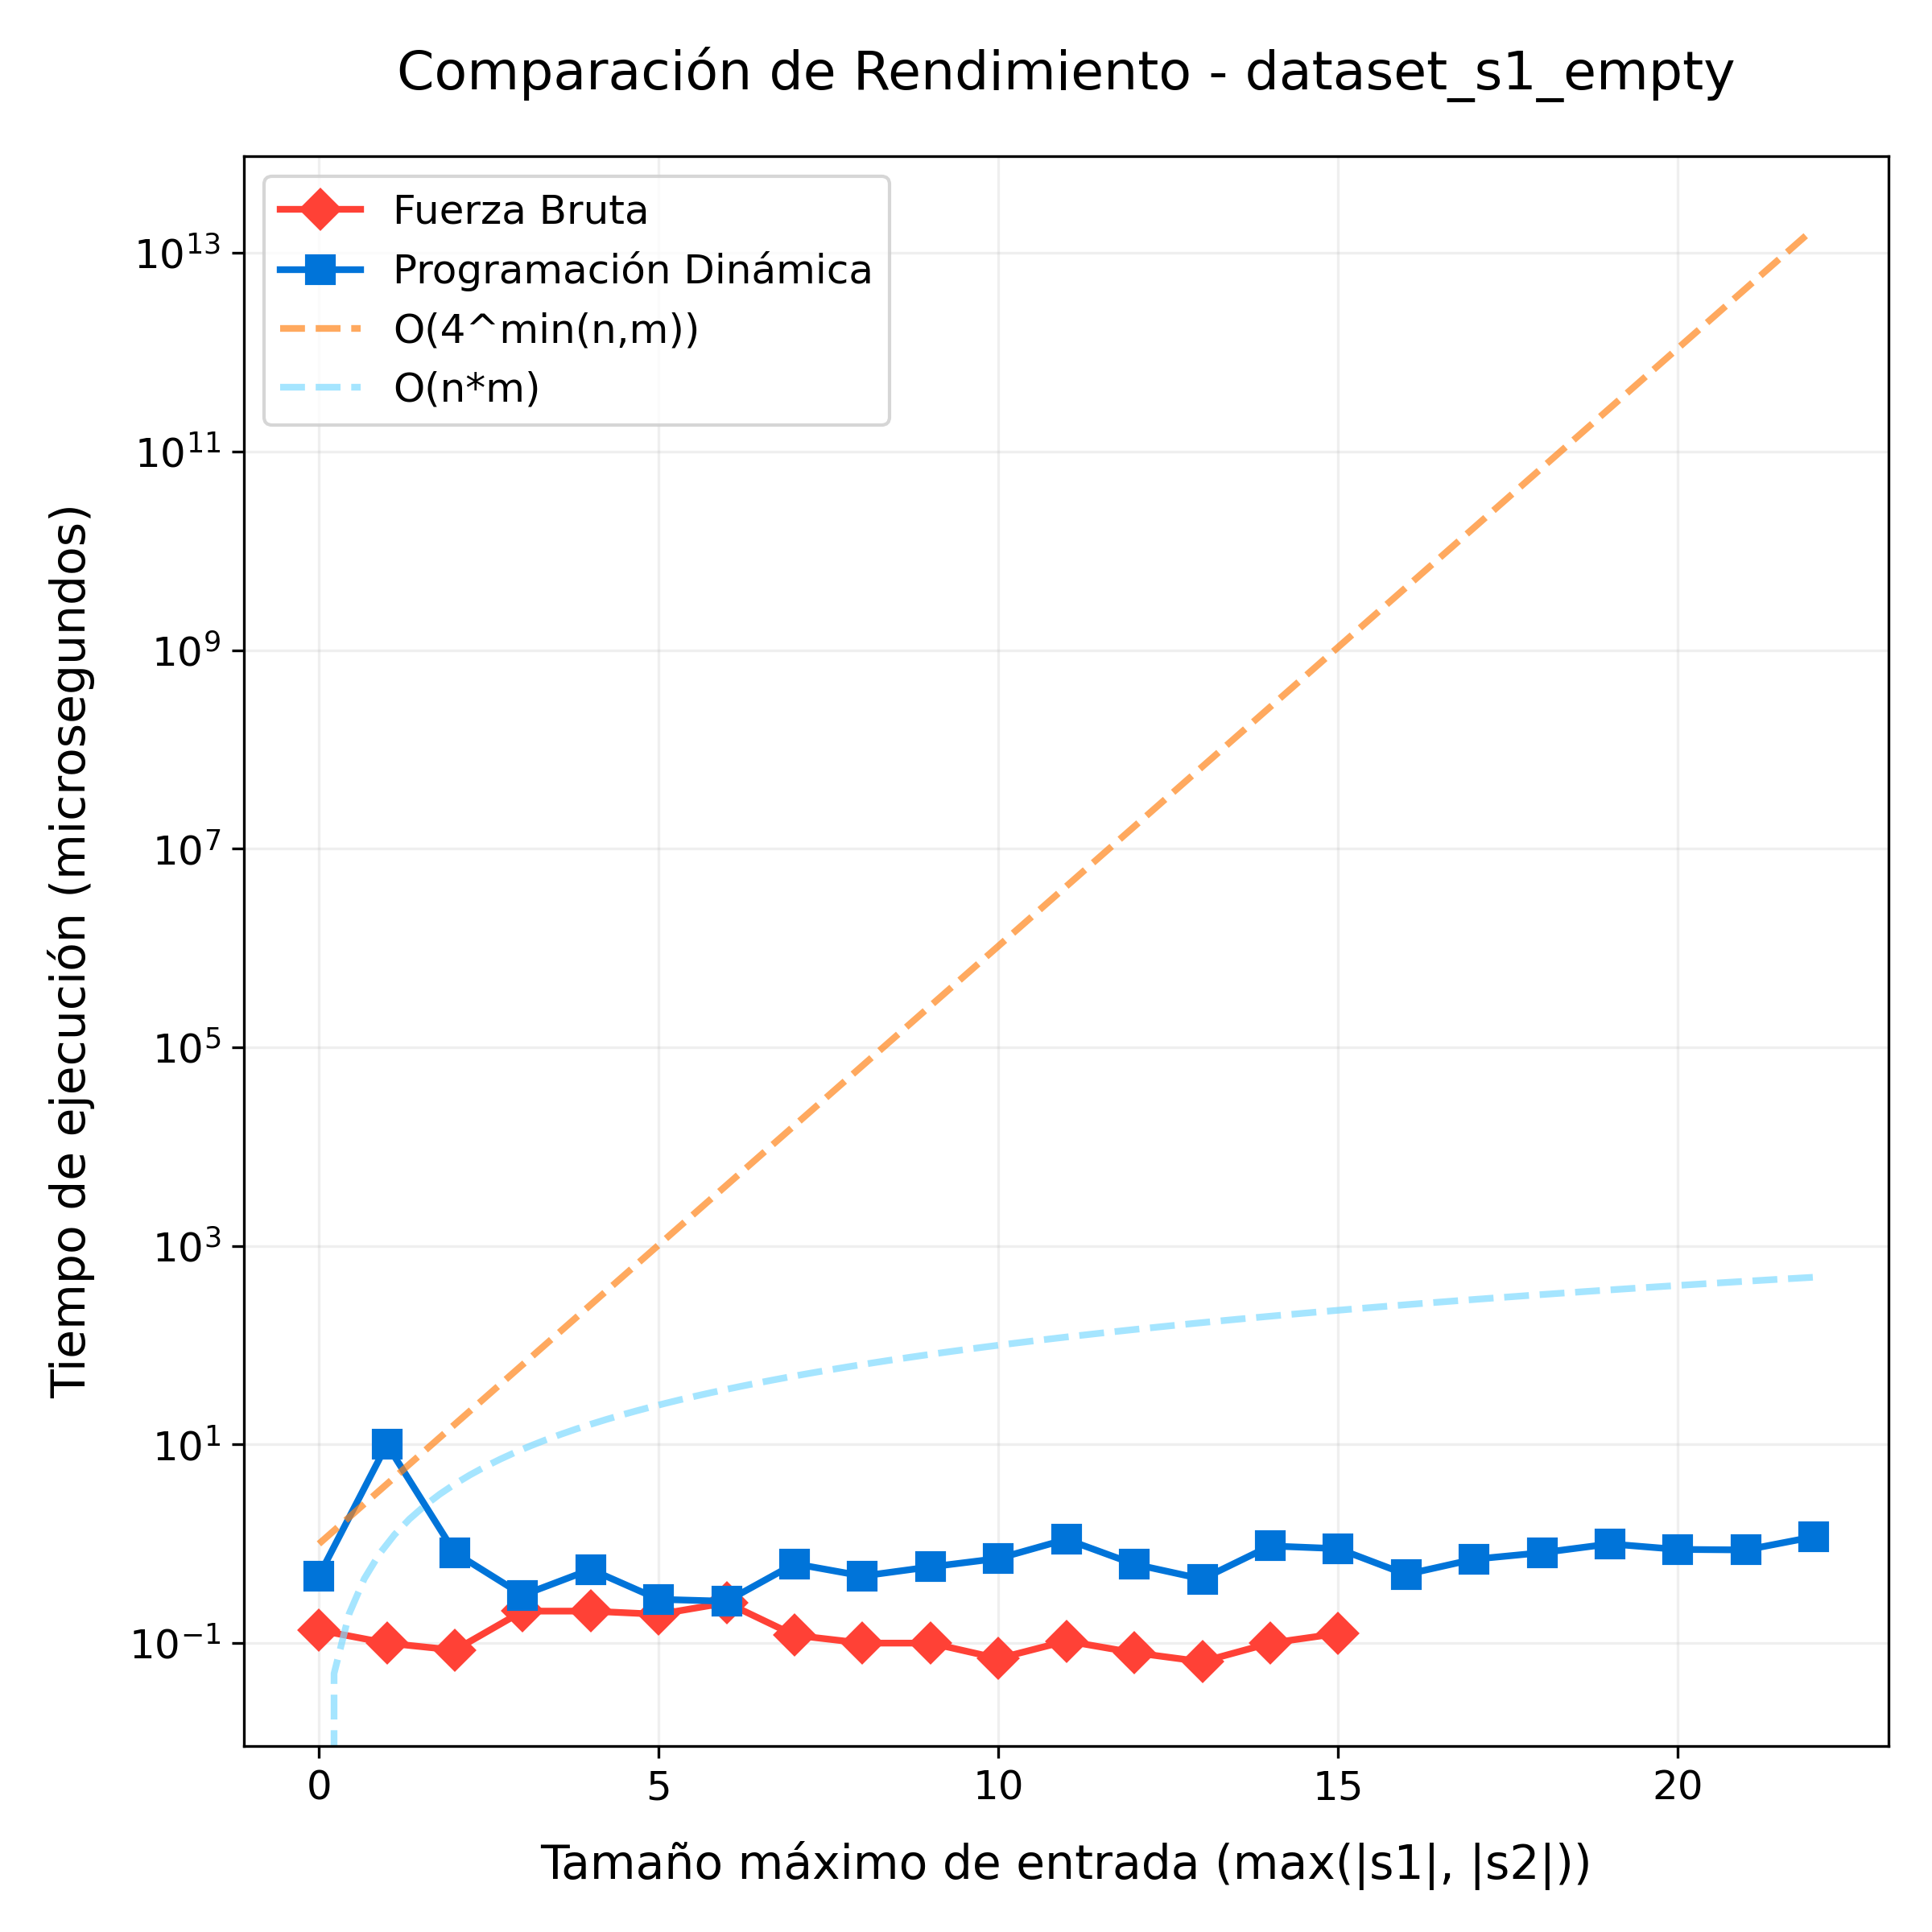
\includegraphics[width=\textwidth]{images/comparacion_dataset_s1_empty.png}
    \end{minipage}%
    \begin{minipage}[t]{0.5\textwidth}
        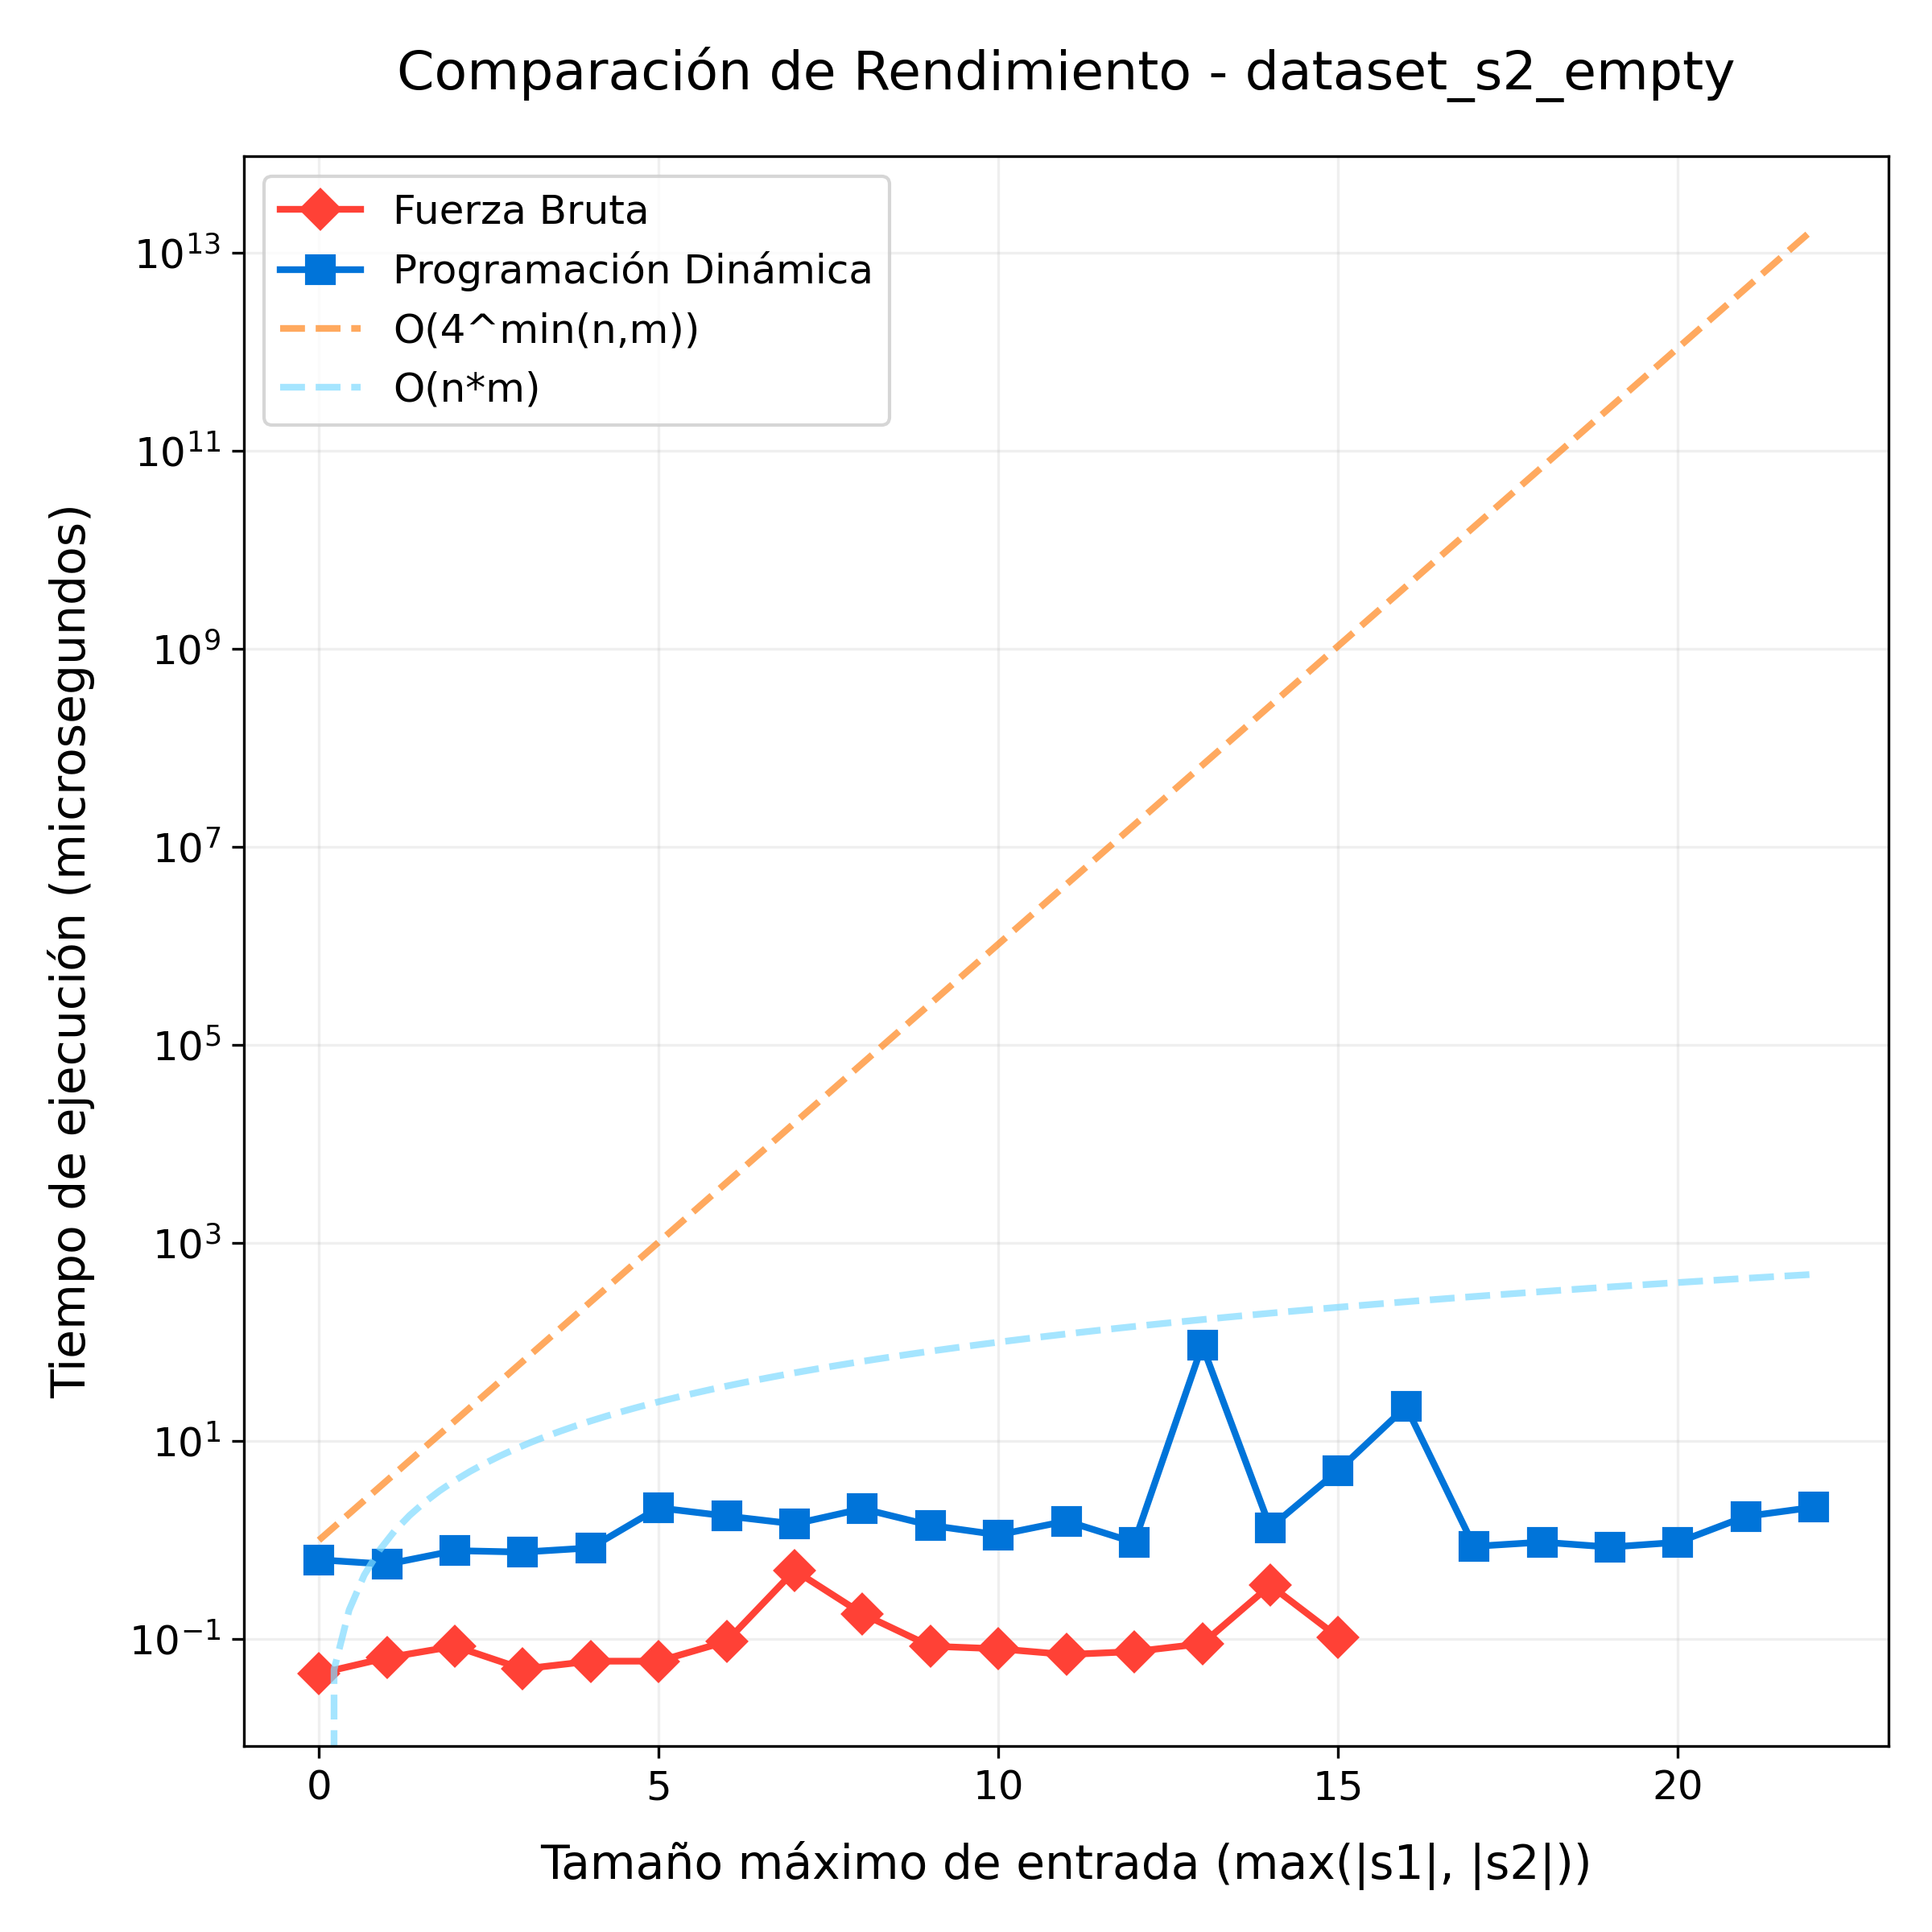
\includegraphics[width=\textwidth]{images/comparacion_dataset_s2_empty.png}   \end{minipage}%
    \caption{Comparación de rendimiento en datasets 1 y 2.}
    \label{fig:dataset1_2}
\end{figure}

En la Figura 1 podemos ver como, si bien el algoritmo DP presenta un coportamiento esperado en base a su complejidad temporal, 
su contraparte de BF se aleja considerablemente de la teoría. Esto, de hecho, lo esperábamos desde la definición del algoritmo, 
ya que para estos datasets nuestra solución cae constantemente en un caso base, realizando exclusivamente operaciones de adición hasta 
recorrer el string no vacío, superando así en rendimiento incluso al enfoque DP.  

\begin{figure}[H]
    \centering
    \begin{minipage}[t]{0.5\textwidth}
        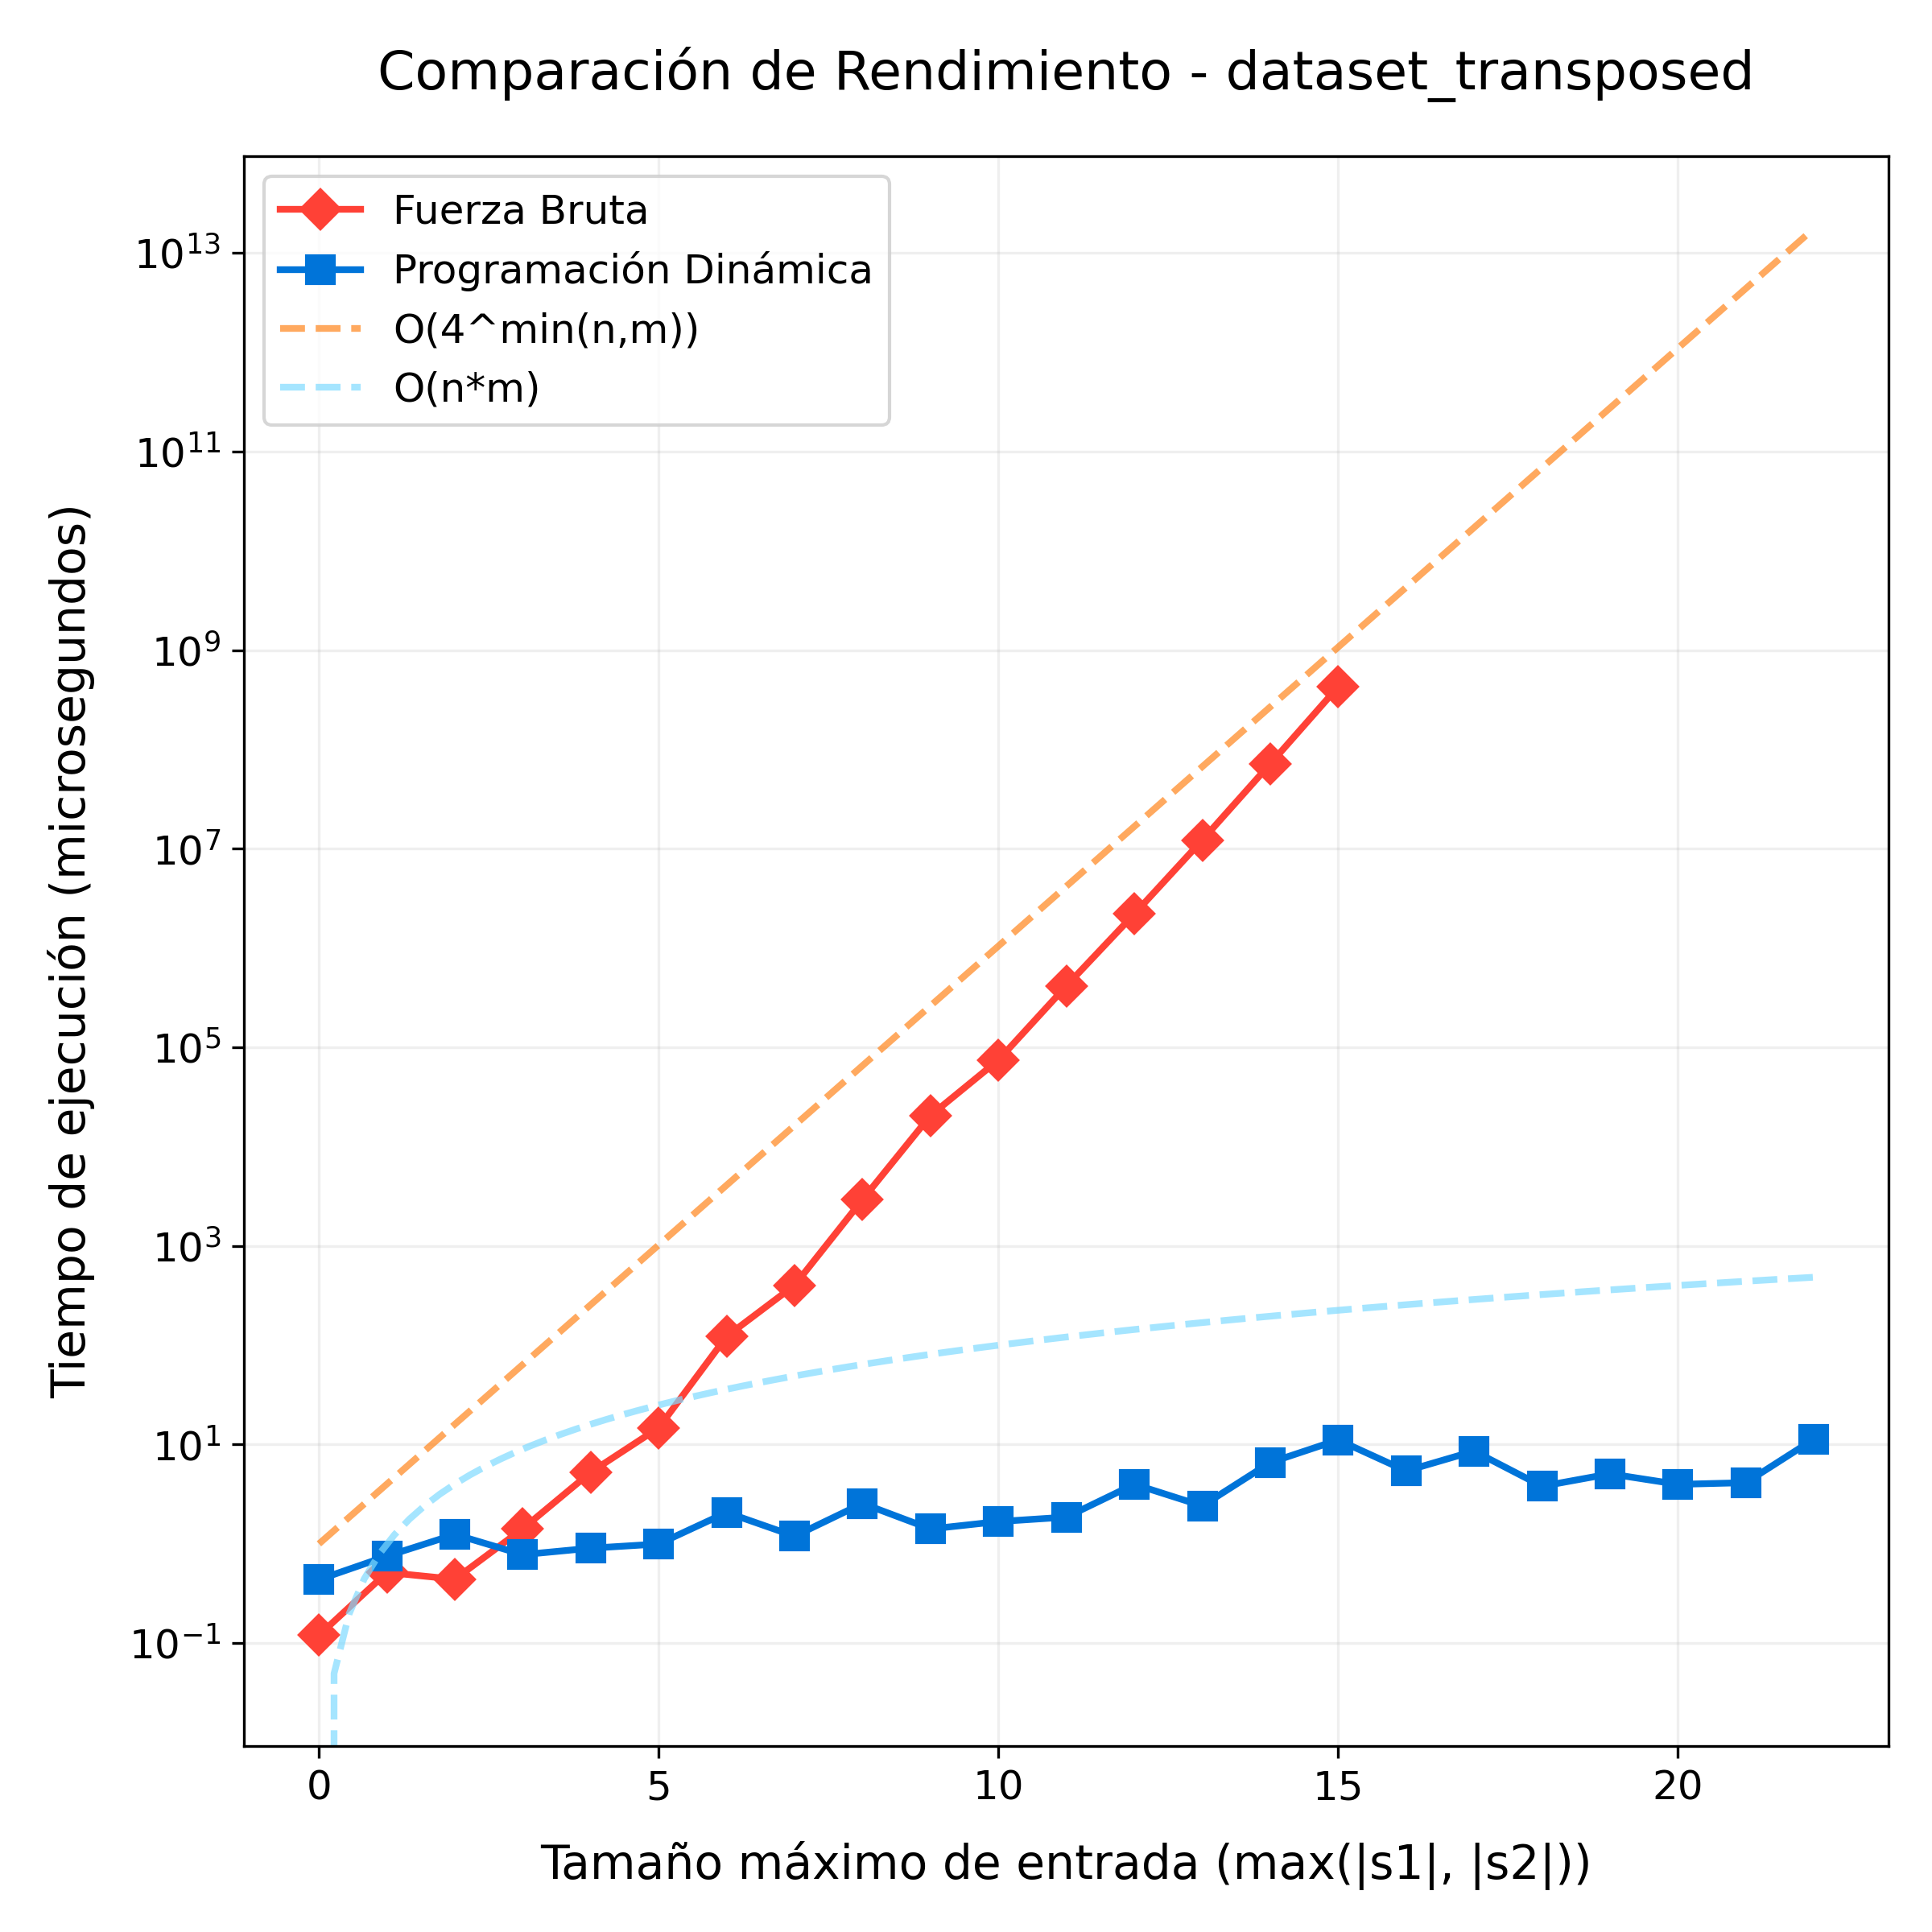
\includegraphics[width=\textwidth]{images/comparacion_dataset_transposed.png}   
    \end{minipage}%
    \begin{minipage}[t]{0.5\textwidth}
        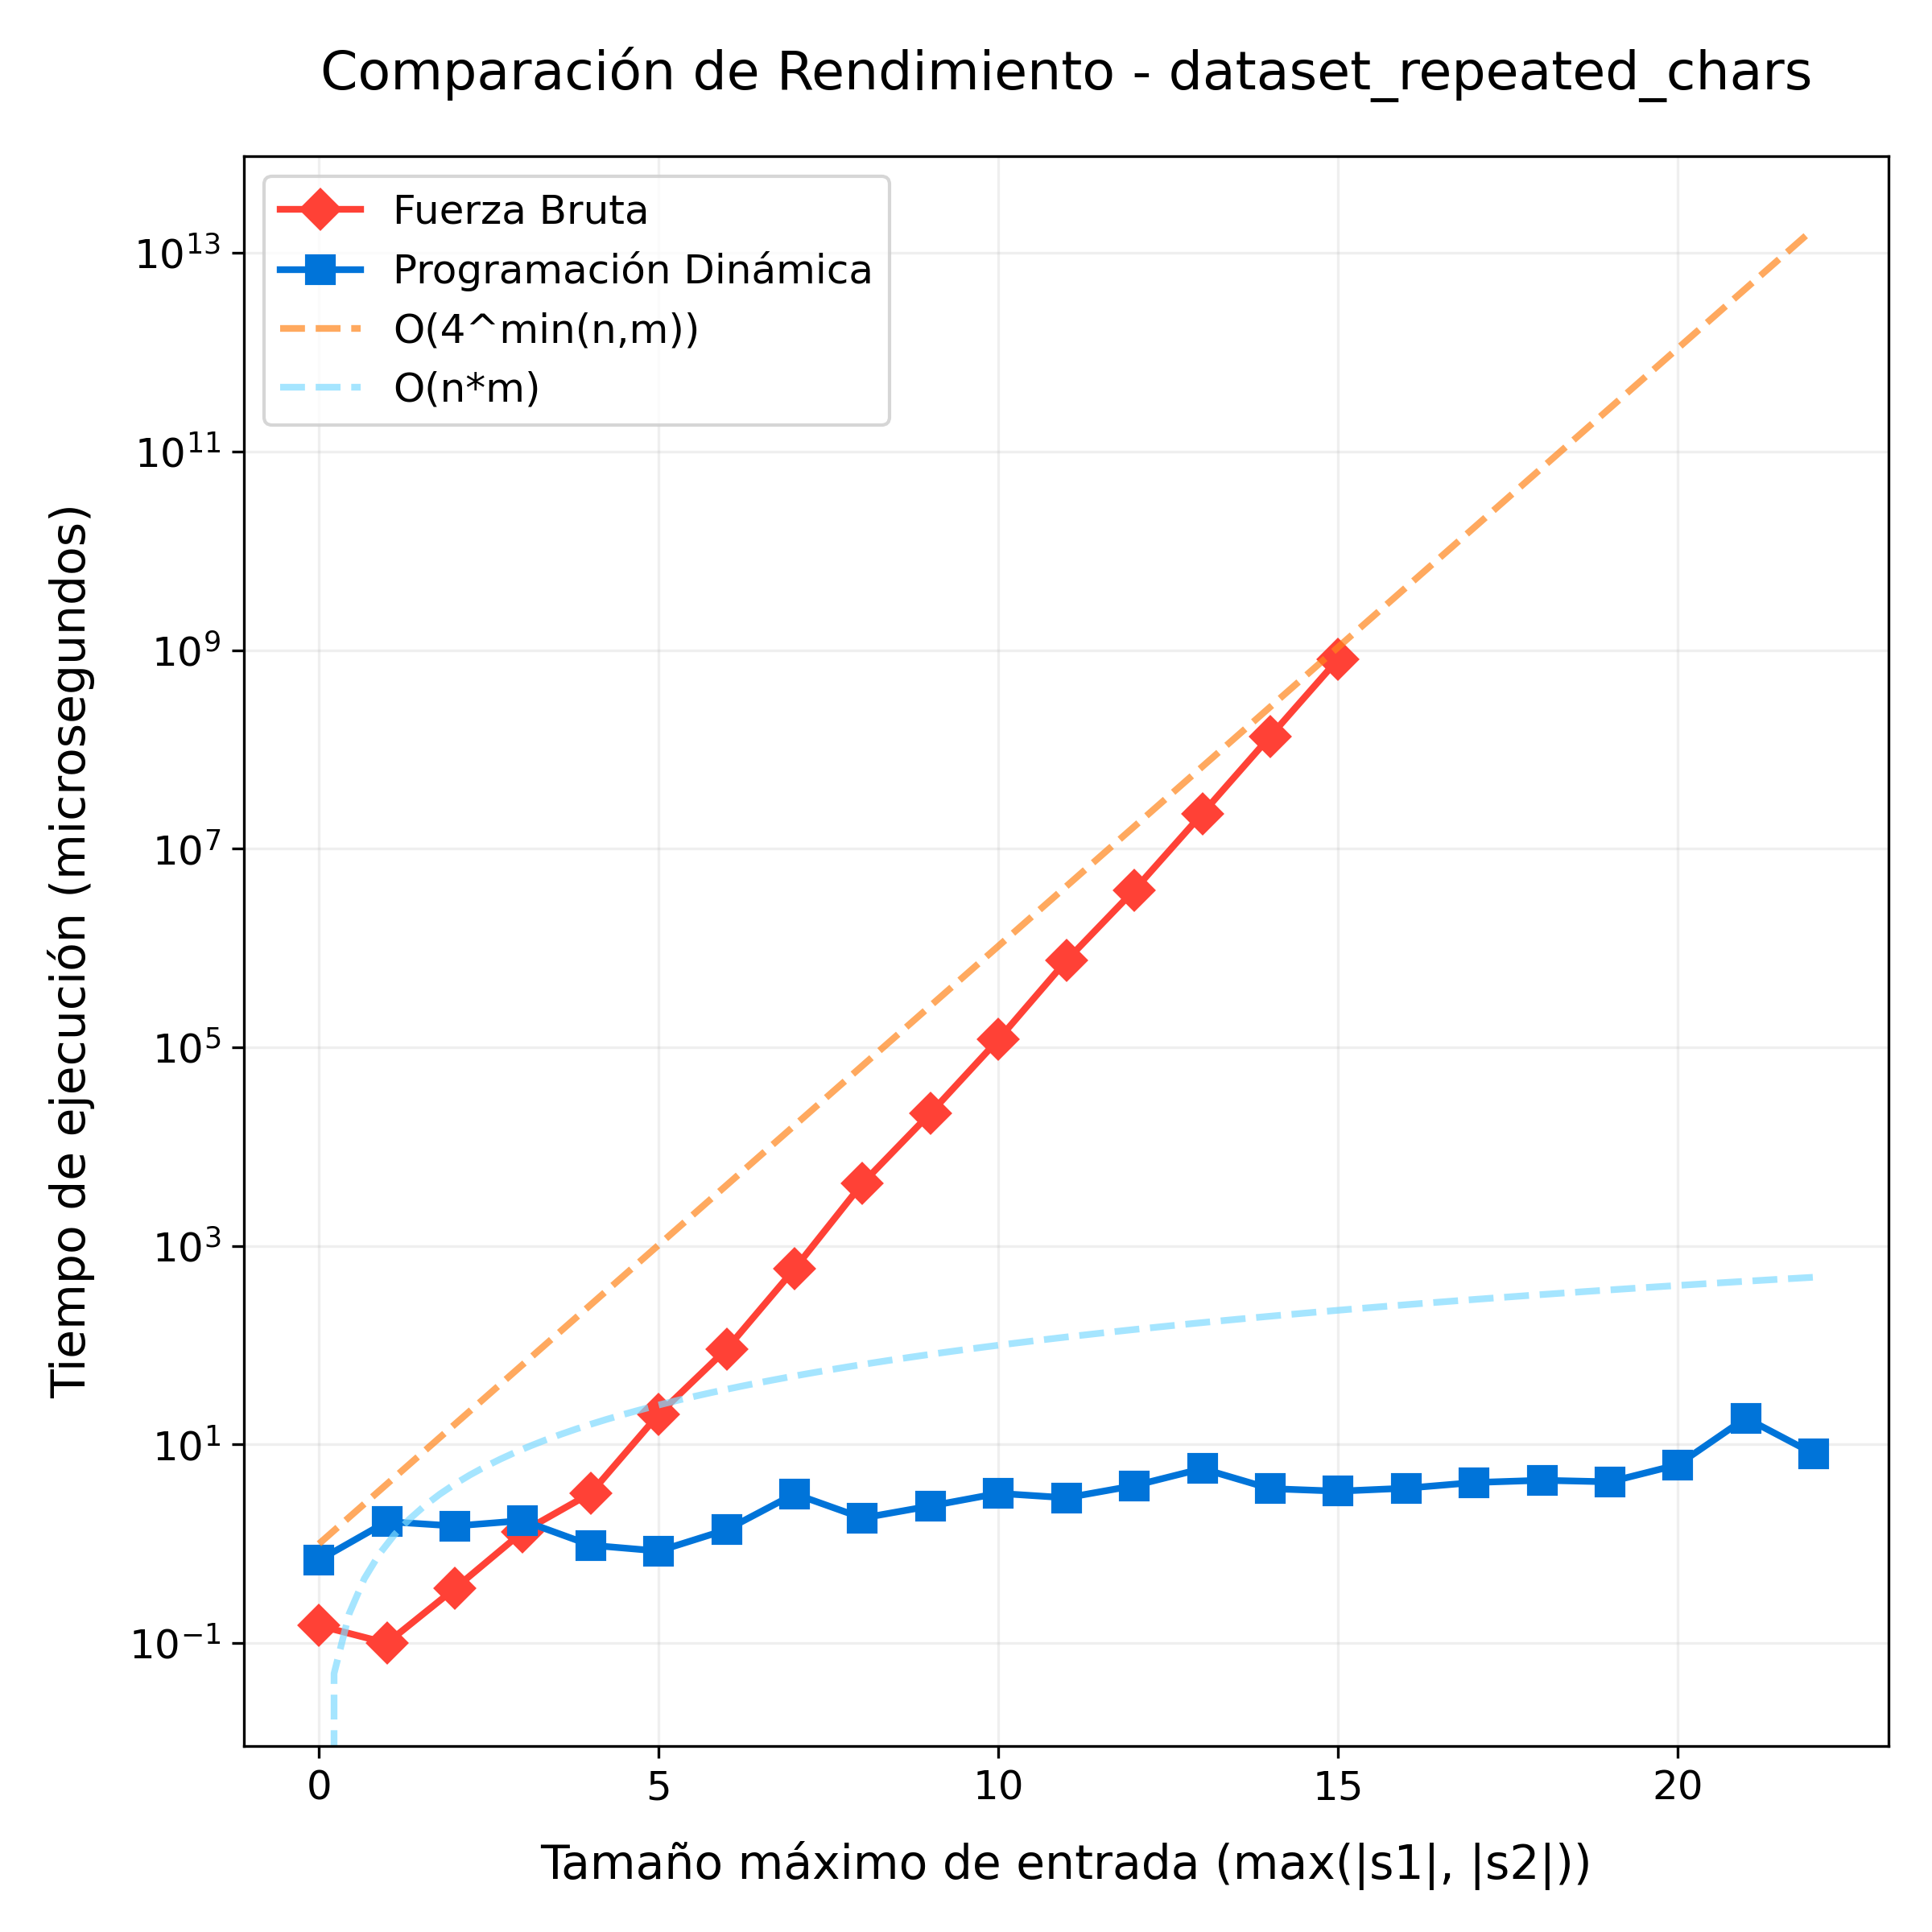
\includegraphics[width=\textwidth]{images/comparacion_dataset_repeated_chars.png} \end{minipage}%
    \caption{Comparación de rendimiento en datasets 3 y 4.}
    \label{fig:dataset3_4}
\end{figure}

En la Figura 2, vemos que DP no cambia, pero BF sufre las consecuencias de su complejidad exponencial, esta vez siguiendo la linea de tendencia esperada según el cálculo 
teórico planteado previamente.

\begin{figure}[H]
    \centering
    \begin{minipage}[t]{0.5\textwidth}
        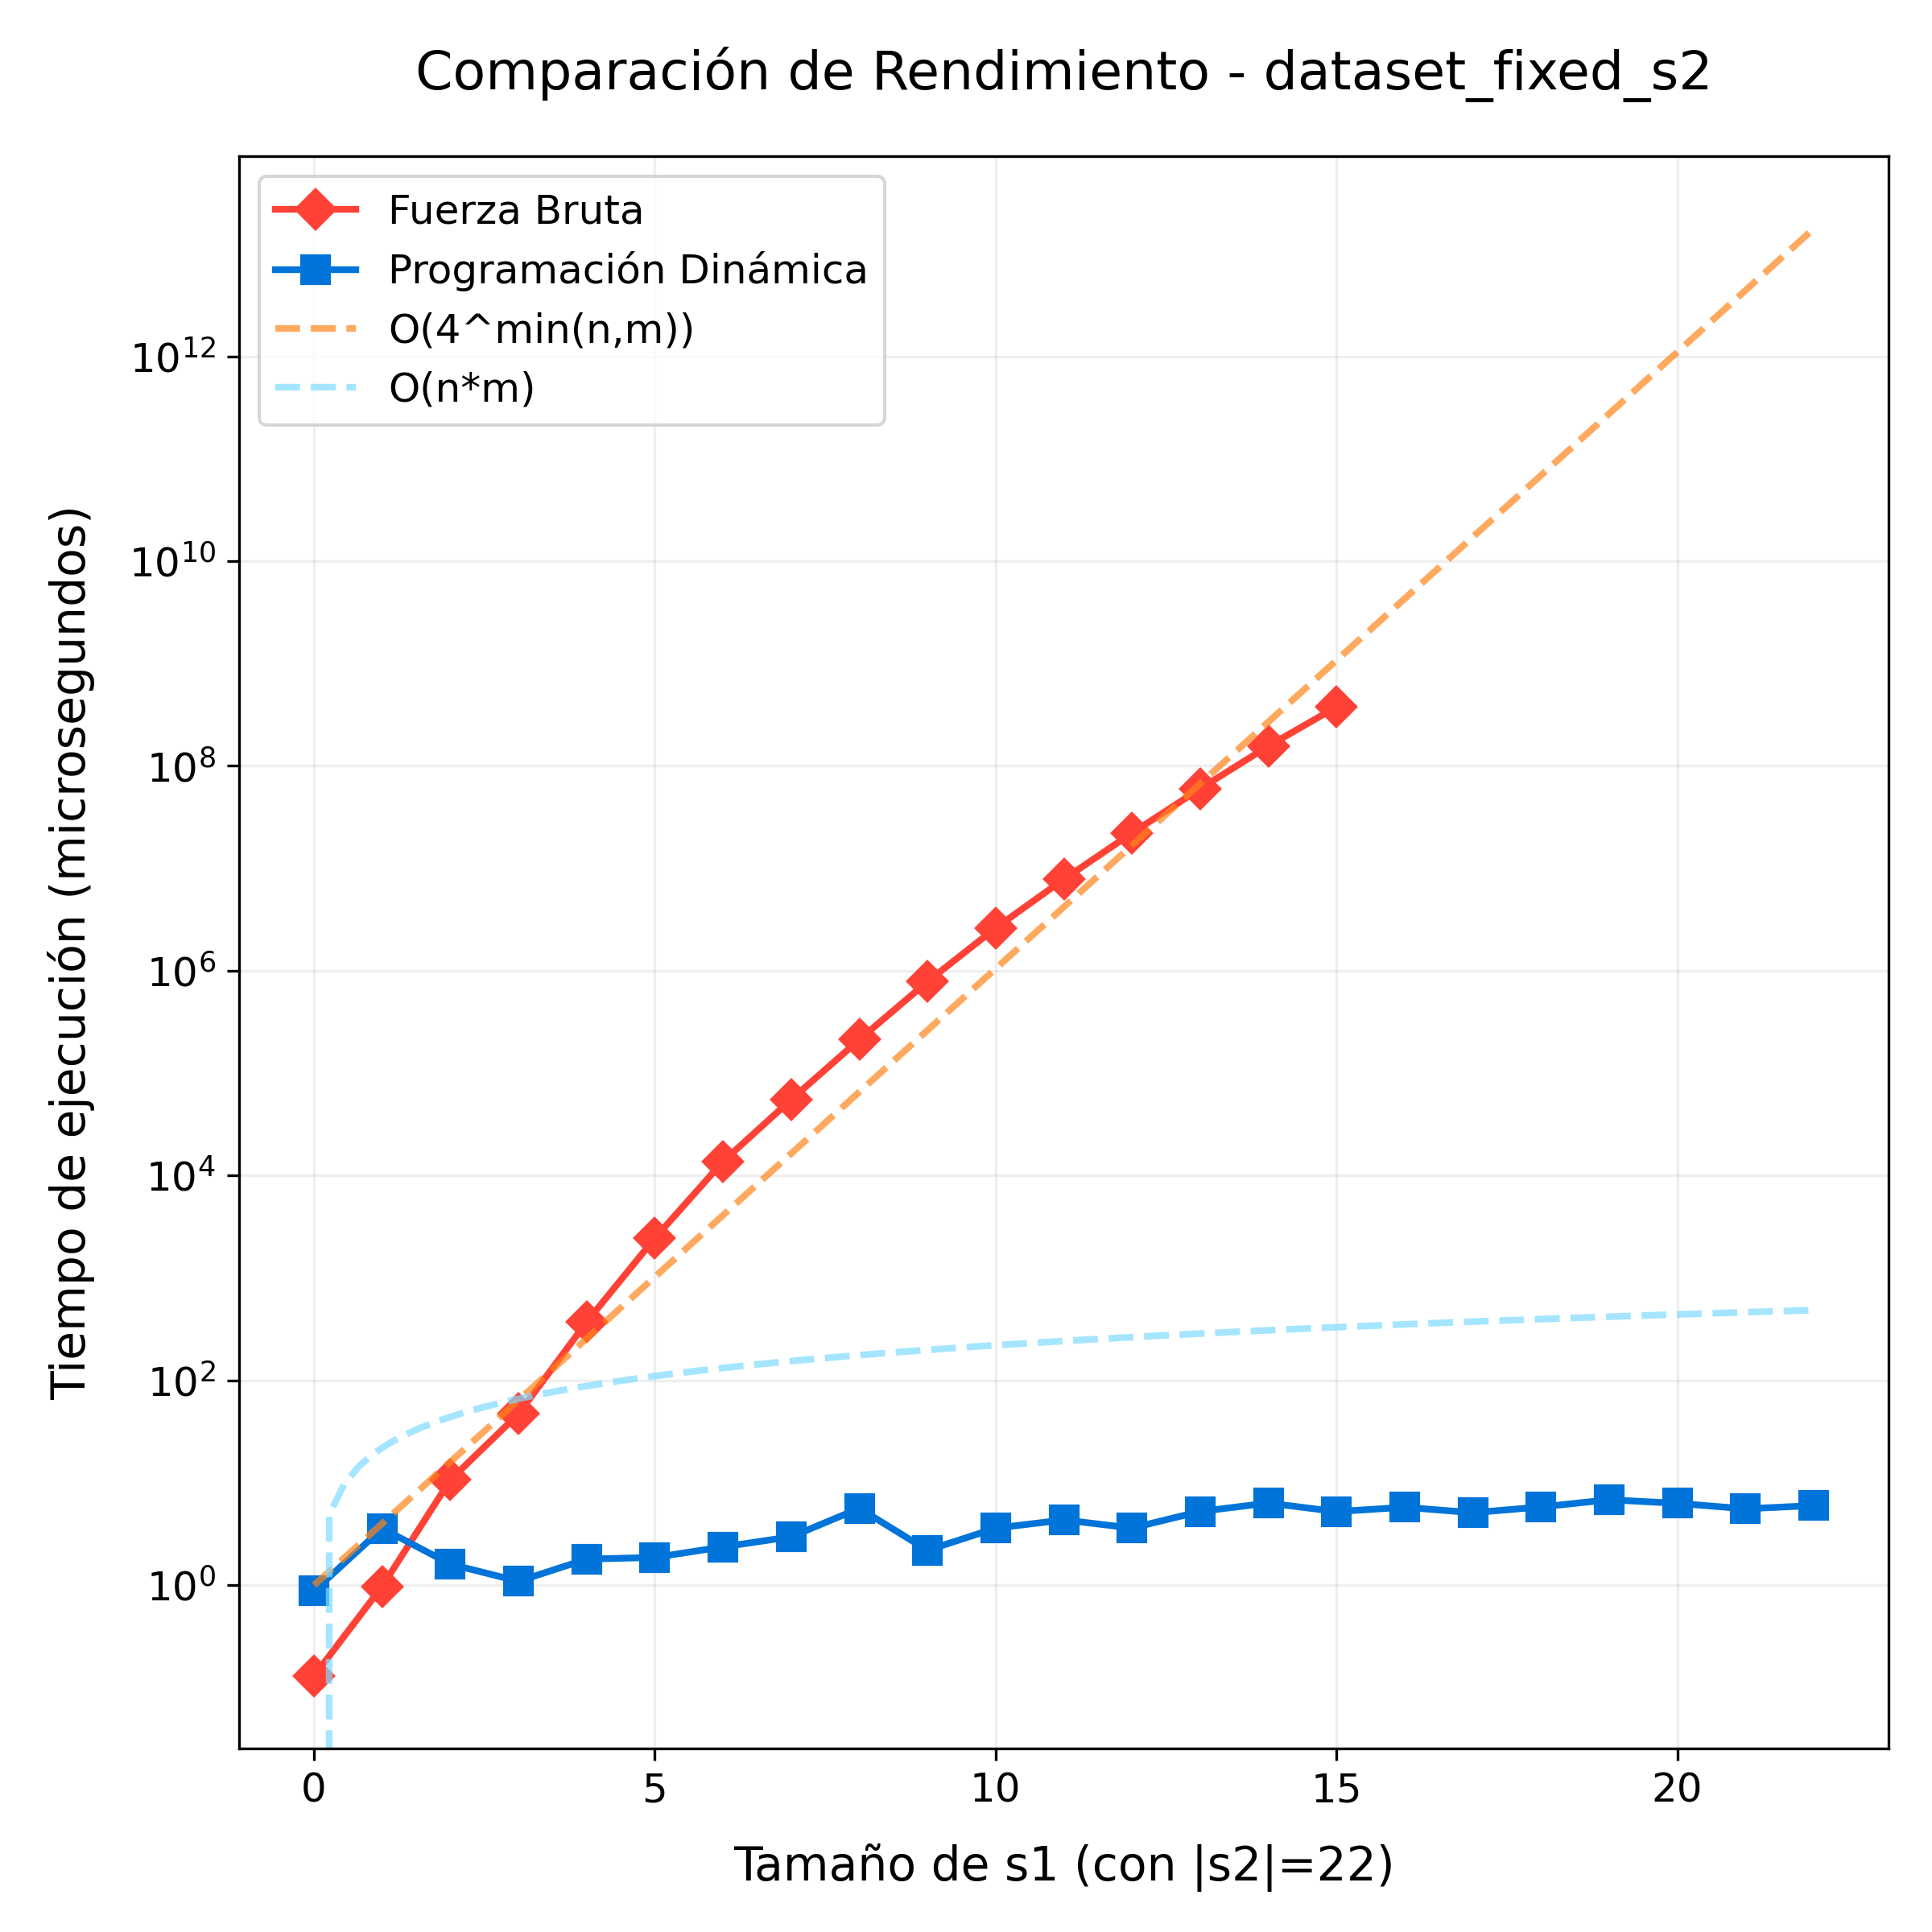
\includegraphics[width=\textwidth]{images/comparacion_dataset_fixed_s2.png}  
    \end{minipage}%
    \caption{Rendimiento dataset 5}
    \label{fig:dataset5_general_memoria}
\end{figure}

En la Figura 3 podemos ver nuevamente el comportamiento exponencial esperado de BF y como DP se mantiene bajo su curva de complejidad. 
Si nos fijamos, bajo este dataset, BF presenta un rendimiento aún peor que en los anteriores. Esto se debe a que s2, al ser constantemente de 
largo máximo, provoca que el tiempo de ejecución aumente con respecto a los largos variables de los datasets anteriores. 

\begin{figure}[H]
    \centering
        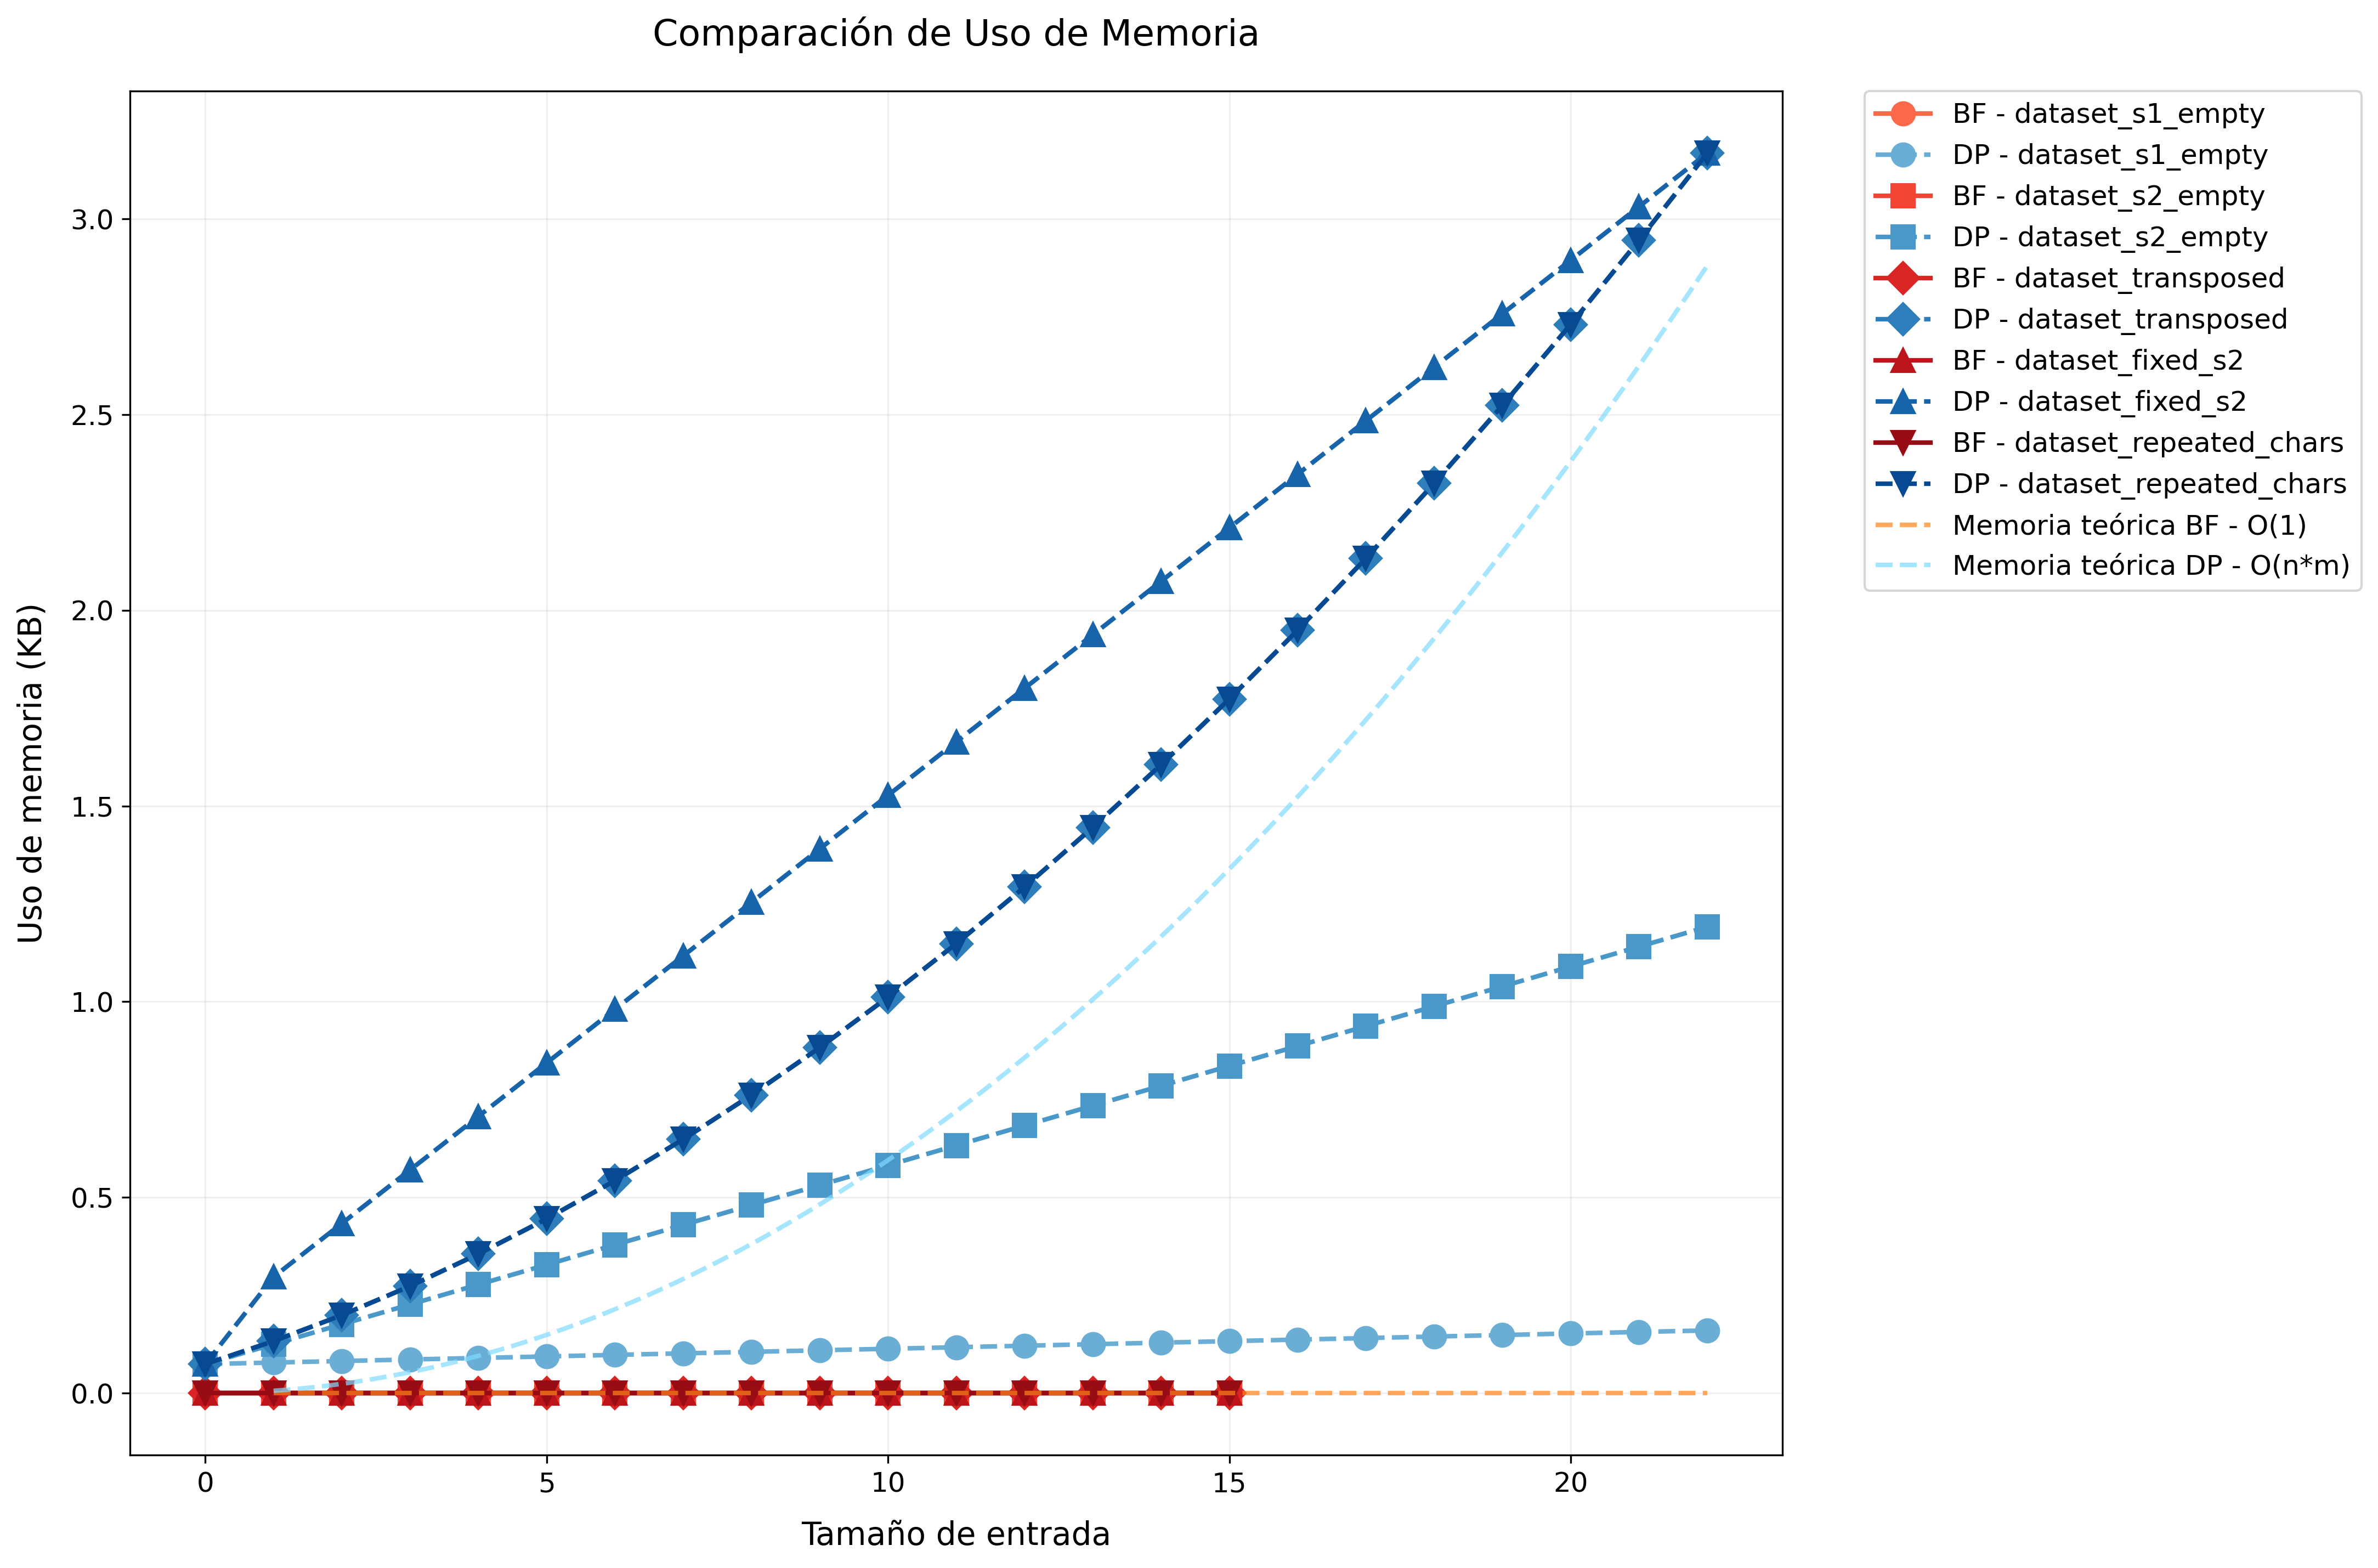
\includegraphics[width=\textwidth]{images/comparacion_memoria.png}
    \caption{Comparación general de uso de memoria}
    \label{fig:general_memoria}
\end{figure}

En la Figura 4 vemos un gráfico general del uso de memoria de cada algoritmo dependiendo del dataset. Podemos notar que para el primer dataset, 
DP ocupa una mínima cantidad de memoria, ya que solo tabula un arreglo. Las mediciones superiores muestran un coportamiento acorde a 
el cálculo teórico, presentando un crecimiento cuadrático. La medición más extravagante es la del dataset 2, es curioso ver que no se comporta como 
su contraparte de s1 vacío (dataset 1). Esto se debe a que para este caso, en vez de solo tabular un arreglo, DP tabula m arreglos de tamaño 1, 
eso explica la considerable diferencia con el dataset 1 pero que tampoco crece de manera cuadrática como el resto de casos. Por su parte, BF se mantiene 
nulo en el uso de memoria, ya que es un algoritmo in-place.

\begin{figure}[H]
    \centering
        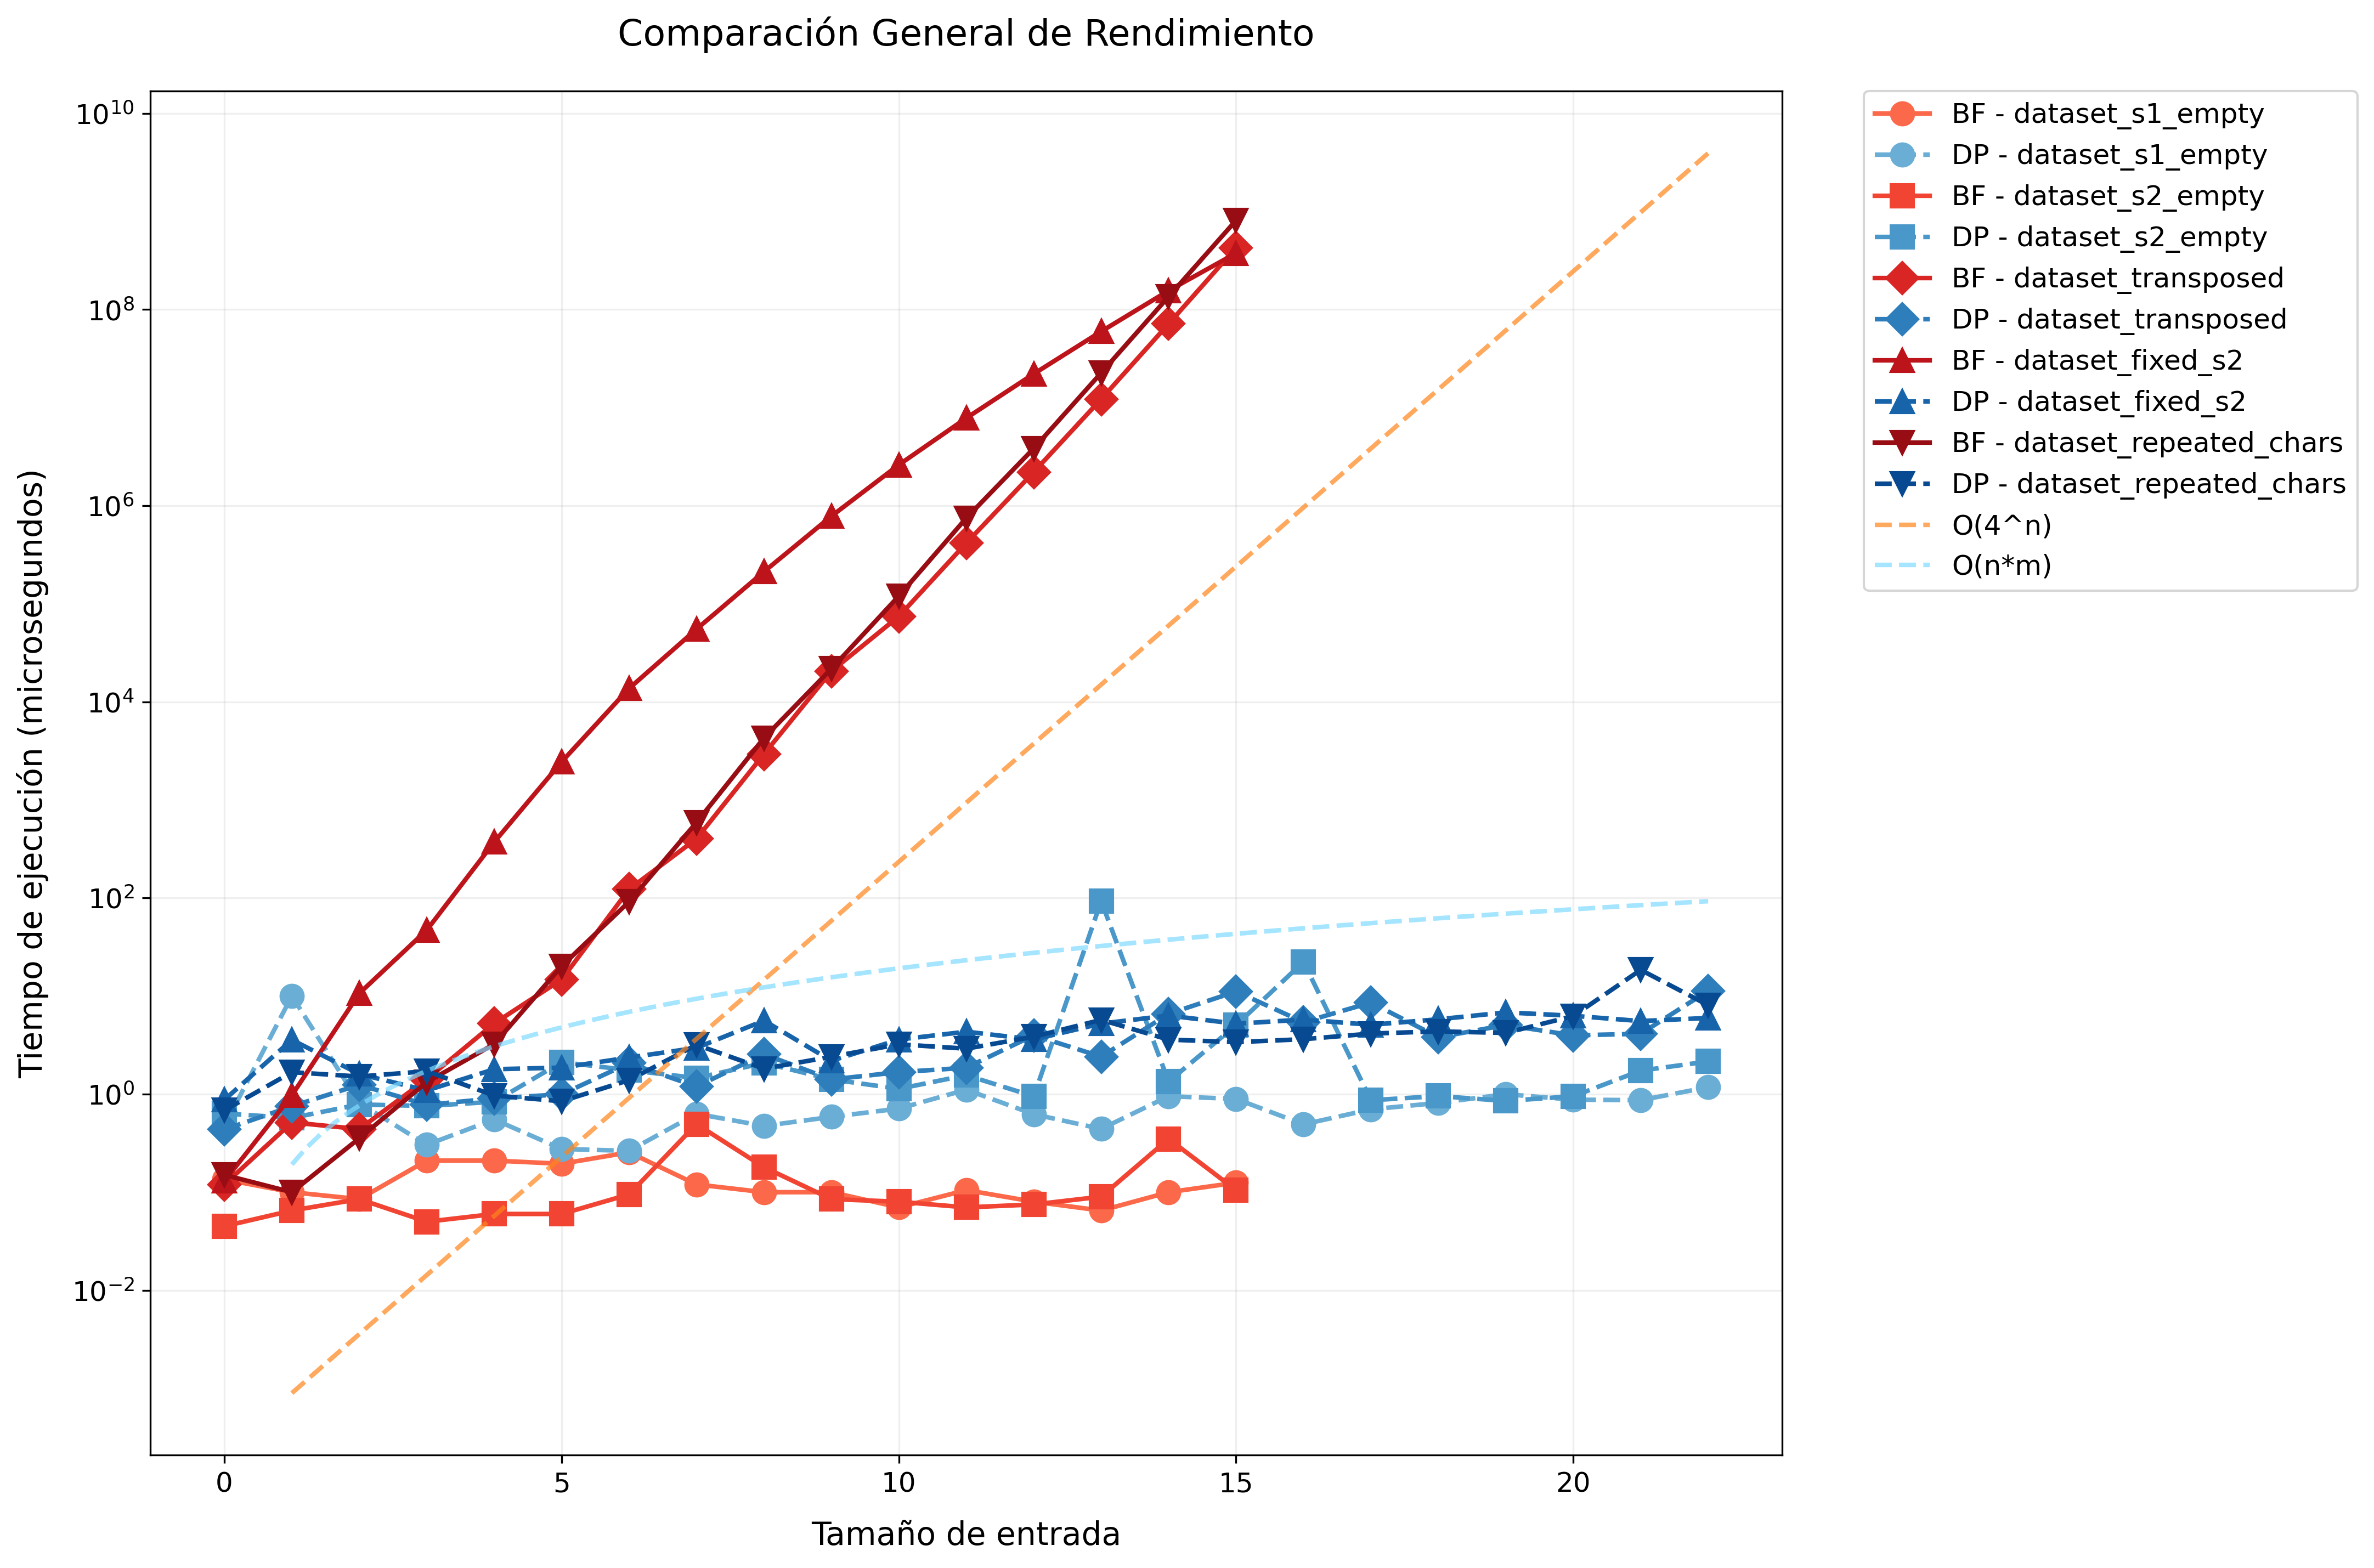
\includegraphics[width=\textwidth]{images/comparacion_general.png}   
    \caption{Comparación general de rendimiento}
    \label{fig:general}
\end{figure}

La Figura 5 presenta una comparación entre todas las mediciones de rendimiento vistas previamente. Podemos ver, como en los datasets 1 y 2, gracias a los casos base, BF 
presentan el mayor rendimiento de todos. Tambien, como en todas y cada una de las mediciones DP respeta su línea teórica, presentando un rendimiento excepcional que supera 
considerablemente las ejecuciones no particulares de BF. Para finalizar, se ve claramente como para los datasets 3, 4 y 5, BF tiene un crecimiento exponencial, siguiendo 
el ratio de la linea teórica, también podemos notar que nuestras predicciones de peor caso planteadas al diseñar el algoritmo eran correctas, ya que el peor tiempo de ejecución 
pertenece a BF en el \textbf{dataset 4 : repeated chars}, un dataset diseñado específicamente para permitir que en todas las llamadas del algoritmo se pueda considerar la opción de 
transponer, maximizando el número de llamadas recursivas, de esta forma logrando un peor rendimiento. 






\newpage
\section{Conclusiones}
\begin{mdframed}
    \textbf{La extensión máxima para esta sección es de 1 página.}
\end{mdframed}

La conclusión de su informe debe enfocarse en el resultado más importante de su trabajo. No se trata de repetir los puntos ya mencionados en el cuerpo del informe, sino de interpretar sus hallazgos desde un nivel más abstracto. En lugar de describir nuevamente lo que hizo, muestre cómo sus resultados responden a la necesidad planteada en la introducción.

\begin{itemize}
    \item  No vuelva a describir lo que ya explicó en el desarrollo del informe. En cambio, interprete sus resultados a un nivel superior, mostrando su relevancia y significado.
    \item Aunque no debe repetir la introducción, la conclusión debe mostrar hasta qué punto logró abordar el problema o necesidad planteada en el inicio. Reflexione sobre el éxito de su análisis o experimento en relación con los objetivos propuestos.
    \item No es necesario restablecer todo lo que hizo (ya lo ha explicado en las secciones anteriores). En su lugar, centre la conclusión en lo que significan sus resultados y cómo contribuyen al entendimiento del problema o tema abordado.
    \item No deben centrarse en sí mismos o en lo que hicieron durante el trabajo (por ejemplo, evitando frases como "primero hicimos esto, luego esto otro...").
    \item Lo más importante es que no se incluyan conclusiones que no se deriven directamente de los resultados obtenidos. Cada afirmación en la conclusión debe estar respaldada por el análisis o los datos presentados. Se debe evitar extraer conclusiones generales o excesivamente amplias que no puedan justificarse con los experimentos realizados.
\end{itemize}


\newpage

\section{Condiciones de entrega}
% Condiciones generales de tareas de Algoritmos y Complejidad, 20231
  \begin{itemize}
  \item
    La tarea se realizará \tca{individualmente}
    (esto es grupos de una persona),
    sin excepciones.
  \item
    La entrega debe realizarse vía \url{http://aula.usm.cl}
    en un \tca{tarball} en el área designada al efecto,
    en el formato \tca{\texttt{tarea-\tnum-{rol}.tar.gz}}
    (\texttt{rol} con dígito verificador y sin guión).

    Dicho \tca{tarball} debe contener las fuentes en \LaTeXe{}
    (al menos \tca{\texttt{tarea-\tnum.tex}})
    de la parte escrita de su entrega,
    además de un archivo \tca{\texttt{tarea-\tnum.pdf}},
    correspondiente a la compilación de esas fuentes.
  \item Si se utiliza algún código, idea, o contenido extraído de otra fuente, este \textbf{debe} ser citado en el lugar exacto donde se utilice, en lugar de mencionarlo al final del informe. 
  \item
    Asegúrese que todas sus entregas tengan sus datos completos:
    número de la tarea, ramo, semestre, nombre y rol.
    Puede incluirlas como comentarios en sus fuentes \LaTeX{}
    (en \TeX{} comentarios son desde \% hasta el final de la línea)
    o en posibles programas.
    Anótese como autor de los textos.
 
  \item
    Si usa material adicional al discutido en clases,
    detállelo.
    Agregue información suficiente para ubicar ese material
    (en caso de no tratarse de discusiones con compañeros de curso
     u otras personas).
  \item No modifique \texttt{preamble.tex}, \texttt{tarea\_main.tex}, \texttt{condiciones.tex}, estructura de directorios, nombres de archivos, configuración del documento, etc. Sólo agregue texto, imágenes, tablas, código, etc. En el códigos funte de su informe, no agregue paquetes, ni archivos .tex (a excepción de que agregue archivos en \texttt{/tikz}, donde puede agregar archivos .tex con las fuentes de gráficos en \texttt{TikZ}).

\ifprograms
  \item
    Su programa ejecutable debe llamarse \tca{\texttt{tarea\tnum}},
    de haber varias preguntas solicitando programas,
    estos deben llamarse usando el número de la pregunta,
    como \tca{\texttt{tarea\tnum-1}},
    \tca{\texttt{tarea\tnum-2}},
    etc.
    Si hay programas compilados, con en este caso,
    incluya una \tca{\texttt{Makefile}}
    que efectúe las compilaciones correspondientes.

    Los programas se evalúan según que tan claros
    (bien escritos)
    son, si se compilan y ejecutan sin errores o advertencias según corresponda.
    Parte del puntaje es por ejecución correcta con casos de prueba.
    Si el programa no se ciñe a los requerimientos de entrada y salida,
    la nota respectiva es cero.
\fi    
  \item
    %La entrega debe realizarse dentro del plazo indicado en \url{http://aula.usm.cl}:
    La fecha límite de entrega es el día \tca{10 de noviembre de 2024}.

    \begin{center}
        \Large{
          \textbf{NO SE ACEPTARÁN TAREAS FUERA DE PLAZO}.
        }
        \normalsize
    \end{center}
     
    
  \item
    Nos reservamos el derecho de llamar a interrogación
    sobre algunas de las tareas entregadas.
    En tal caso,
    la nota de la tarea será la obtenida en la interrogación.
    \begin{center}
      \Large{
        \textbf{NO PRESENTARSE A UN LLAMADO A INTERROGACIÓN SIN JUSTIFICACIÓN PREVIA SIGNIFICA AUTOMÁTICAMENTE NOTA 0.}
      }
    \end{center}
    
  \end{itemize}

%%% Local Variables:
%%% mode: latex
%%% ispell-local-dictionary: "spanish"
%%% End:

  
% LocalWords:  tarball tar gz pdf min entregable Makefile puntaje
% LocalWords:  Moodle

\newpage
\appendix


\section{Apéndice 1}
Aquí puede agregar tablas, figuras u otro material que no se incluyó en el cuerpo principal del documento, ya que no constituyen elementos centrales de la tarea. Si desea agregar material adicional que apoye o complemente el análisis realizado, puede hacerlo en esta sección.

\begin{mdframed} 
    Esta sección es solo para material adicional. El contenido aquí no será evaluado directamente, pero puede ser útil si incluye material que será referenciado en el cuerpo del documento. Por lo tanto, asegúrese de que cualquier elemento incluido esté correctamente referenciado y justificado en el informe principal.
 \end{mdframed}


 
\printbibliography

\end{document}


